% !BIB program = biber
\ifdefined\paperversion
\documentclass[a4paper,titlepage,twoside,openright]{report}
\else
\documentclass[a4paper,titlepage]{report}
\fi
\usepackage[utf8]{inputenc}
% Default looks better
% \usepackage[a4paper,top=2cm,bottom=2cm,inner=2.5cm,outer=6cm]{geometry}
% Font FiraSans - see http://www.tug.dk/FontCatalogue/firasansnewtxsf/
\usepackage[T1]{fontenc}
\usepackage[sfdefault,scaled=.85]{FiraSans}
\usepackage{newtxsf}
\usepackage{verbatim}
%
% Watermark - remove when complete
\usepackage{draftwatermark}
\SetWatermarkText{Draft}
\SetWatermarkScale{0.2}
%
% showframe - comment out usually
%\usepackage{showframe}
%
\ifdefined\paperversion
\usepackage[pdftex,
  pdftitle={BGP for networks who peer},
  pdflang={en-US},
  pdfauthor={Wolfgang Tremmel},
  pdfcreator={DE-CIX Academy},
  pdfsubject={BGP},
  pdfdisplaydoctitle=true,  hidelinks
%
% For printing,   hidelinks
% For online,   % hidelinks
%
%  hidelinks
  ]{hyperref}
\else
\usepackage[pdftex,
  pdftitle={BGP for networks who peer},
  pdflang={en-US},
  pdfauthor={Wolfgang Tremmel},
  pdfcreator={DE-CIX Academy},
  pdfsubject={BGP},
  pdfdisplaydoctitle=true, % hidelinks
%
% For printing,   hidelinks
% For online,   % hidelinks
%
%  hidelinks
  ]{hyperref}
\fi
\usepackage[acronym,toc]{glossaries}
\usepackage{parskip}
\usepackage{stackengine}
\usepackage{scalerel}
\usepackage{graphicx}
\usepackage{tabularx}
\usepackage{tabu}
\usepackage{float}
\usepackage{eso-pic}
\usepackage{datetime}
\newdateformat{monthyear}{\monthname~\THEYEAR}
\usepackage{csquotes}
\usepackage{fancyhdr}
\usepackage{xcolor}
\definecolor{lgray}{gray}{0.9}
\usepackage[backend=biber,style=alphabetic,sorting=ynt]{biblatex}
\addbibresource{all-rfcs.bib}
\addbibresource{references.bib}
\floatstyle{boxed}
\restylefloat{figure}
\graphicspath{{img/}{img/Drawings}}
\newcommand\dangersign[1][2ex]{\renewcommand\stacktype{L}\scaleto{\stackon[0.5pt]{\color{red}$\triangle$}{\tiny !}}{#1}}
\newcommand{\ip}[1]{\texttt{#1}}
\newcommand{\rfc}[1]{\cite{rfc#1}}
% Front page picture
\newcommand\TitlePic{%
\put(0,0){%
\parbox[b][\paperheight]{\paperwidth}{%
\vfill
\centering

\includegraphics[width=\paperwidth,height=\paperheight,keepaspectratio,page=2]{./img/Titel_BGP_Lay.pdf}%
\vfill
}}}
\makeglossaries
\glsresetall
\newglossaryentry{Autonomous System}
{
  name=Autonomous System,
  description={is a connected group of one or more IP prefixes run by one
        or more network operators which has a SINGLE and CLEARLY DEFINED
        routing policy}
}
\newacronym[shortplural=ASes]{AS}{AS}{Autonomous System}

\newglossaryentry{Autonomous System Number}
{
  name=Autonomous System Number,
  description={is a 32-bit number uniquely identifying an \gls{Autonomous System}}
}
\newacronym{ASN}{ASN}{Autonomous System Number}

\newglossaryentry{AS Confederation}
{
  name=AS Confederation,
  description={is according to \rfc{5065} a collection of autonomous systems represented and advertised as a single AS number to BGP speakers that are not members of the local BGP confederation.}
}

\newglossaryentry{AS Confederation Identifier}
{
  name=AS Confederation Identifier,
  description={is according to \rfc{5065} an externally visible autonomous system number that identifies a BGP confederation as a whole.}
}

\newacronym{BFD}{BFD}{Bidirectional Forwarding Detection}
\newglossaryentry{bfd}{
name=Bidirectional Forwarding Detection,
description={\glsreset{BFD}\gls{BFD} is a protocol to check if a configured neighbor is alive. For this packets are sent quite rapidly between two systems (rapidly means in the 100ms time range), if no packets are received from the neighbor for a given time, the neighbor is considered to be no longer reachable which is then signaled to other protocols like BGP. BFD is defined in \rfc{5880}, its application on IPv4 and IPv6 is defined in \rfc{5881}. \rfc{5882} is about the general application of BFD and \rfc{5883} describes BFD on multihop paths.}
}


\newacronym{BGP}{BGP}{Border Gateway Protocol}
\newglossaryentry{Border Gateway Protocol}{
  name = Border Gateway Protocol,
  description = {is a distance vector routing protocol used to exchange
  routing information between providers}
}

\newglossaryentry{BGP Attribute}{
  name={BGP Path Attribute},
  description={BGP update messages for prefixes contain not only the AS-Path but also other attributes. These fall into the following four categories:
  \begin{description}
    \item [well-known mandatory:] Needs to be understood by all BGP implementations and must be included in all prefix updates.
    \item [well-known discretionary:] Needs to be understood by all BGP implementations but do not have to be there.
    \item [optional transitive:] Do not have to be there, do not have to be understood by all implementations, but \emph{stay} on the prefix and are forwarded to other BGP speakers (even if not understood)
    \item [optional non-transitive:] Similar, but is not passed along to other BGP speakers
  \end{description}
  }
}

\newacronym{EIGRP}{EIGRP}{Enhanced Interior Gateway Routing Protocol}
\newglossaryentry{Enhanced Interior Gateway Routing Protocol} {
  name =  Enhanced Interior Gateway Routing Protocol,
  description = { is a \gls{IGP} defined by Cisco in the 1980s to distribute
  routing information within a network. It was later openly specified in
  \cite{rfc7868}}
}

\newglossaryentry{default free zone}{
  name = Default Free Zone,
  description = {Part of the Internet where no default route is needed for routing but all routers know all prefixes}
}

\newacronym{EGP}{EGP}{Exterior Gateway Protocol}
\newglossaryentry{Exterior Gateway Protocol}{
  name=Exterior Gateway Protocol,
  description={was a predecessor to BGP. First defined 1982 in \rfc{827} it became obsolete once BGP was widely used (around 1994)}
}

\newglossaryentry{global routing table}{
name = Global Routing Table,
description= {is the table in a router which contains all prefixes currently being routed in the \gls{default free zone} of the Internet}
}

\newacronym{IANA}{IANA}{Internet Assigned Numbers Authority}
\newglossaryentry{Internet Assigned Numbers Authority}{
  name = Internet Assigned Numbers Authority,
  description = {is an entity responsible for all number resources in the Internet. This includes addresses, protocol identifiers, and more}
}

\newacronym{ietf}{IETF}{Internet Engineering Task Force}

\newacronym{IGP}{IGP}{Interior Gateway Protocol}
\newglossaryentry{Interior Gateway Protocol}{
  name = Interior Gateway Protocol,
  description = {is a protocol running inside an Autonomous System to
  distribute the IP addresses of router interfaces}
}

\newacronym{IP}{IP}{Internet Protocol}
\newglossaryentry{Internet Protocol}{
  name={Internet Protocol},
  description={is a protocol responsible for end-to-end communication on the Internet. 
  There are currently two versions in use, named \gls{IPv4} and  \gls{IPv6}
  }}

\newacronym[]{IPv4}{IPv4}{Internet Protocol Version 4}
\newacronym[]{IPv6}{IPv6}{Internet Protocol Version 6}

\newglossaryentry{IS-IS}{
  name = IS-IS,
  description = {(Intermediate System to Intermediate System) is an \gls{IGP} running directly on top of layer 2. It is used
  to distribute interface addresses within a network}
}

\newacronym{LIR}{LIR}{Local Internet Registry}
\newglossaryentry{Local Internet Registry} {
  name = Local Internet Registry,
  plural = Local Internet Registries,
  description = {is an organzation/company which receives IP address resources
  or Autonomous System Numbers as an allocation from a Regional Internet Registry and assigns these
  resources to end users}
}

\newglossaryentry{OSPF}{
  name=Open Shortest Path First,
  description={ is a link state routing protocol. It is used as an \gls{IGP}}
}


\newacronym[longplural={Regional Internet Registries}]{RIR}{RIR}{Regional Internet Registry}
\newglossaryentry{Regional Internet Registry} {
  name=Regional Internet Registry,
  plural=Regional Internet Registries,
  description={is an entity responsible for allocating IP addresses and AS numbers to
    Internet Providers}
}

\newacronym[longplural={Requests for Comment}]{rfc}{RFC}{Request for Comments}


\newacronym{RIP}{RIP}{Routing Information Protocol}
\newglossaryentry{Routing Information Protocol}{
  name=Routing Information Protocol,
  description={is an old and quite obsolete protocol which was used to
  distribute routing information. RIP is no longer in use}
}

\newglossaryentry{RIPE}{
  name = RIPE,
  description = {short for \emph{Réseaux IP Européens}, is the community of network operators in the European, Russian, and Middle Eastern region. See also \gls{RIPE NCC}}
}

\newglossaryentry{RIPE NCC}{
  name = RIPE NCC,
  description = {is the \glsreset{RIR}\gls{RIR} for the European, Russian, and Middle Eastern region}
}

\newglossaryentry{Route Reflector}{
  name=Route Reflector,
  description={is an iBGP speaker which sends \emph{all} prefixes it receives out to its \glspl{Route Reflector Client}}
}

\newglossaryentry{Route Reflector Client}{
  name=Route Reflector Client,
  description={is an iBGP speaking node with usually only one iBGP connection to a \gls{Route Reflector}},
  plural=Route Reflector Clients
}

\newacronym{RTT}{RTT}{Round Trip Time}
\newglossaryentry{Round Trip Time}{name={Round Trip Time},description={is the time measured in seconds or milliseconds it takes from sending out a packet until receiving a reply.}}

\newacronym{TCP}{TCP}{Transmission Control Protocol}
\newglossaryentry{Transmission Control Protocol}{
  name=TCP,
  description={is part of the TCP/IP protocol stack. It is a connection oriented protocol taking care that everything which is sent is also received}
}

\newglossaryentry{MD5}{
name=MD5,
description={is a hash algorithm, used to generate a checksum on given data}
}

\newacronym{TTL}{TTL}{\gls{Time To Live}}
\newglossaryentry{Time To Live}{
name=Time To Live,
description={is a counter in the \gls{IP} header which is decreased every time a packet is forwarded by a router. If this counter hits zero, the packet is discarded and an \gls{ICMP} Time Exceeded message is sent back to the originator of the packet}
}

\newglossaryentry{default-route}{
name=Default Route,
description={is a route which covers every destination for which there is no specific route in the routing table. The destination of the default-route is often called the default destination or the gateway of last resort}
}

\newglossaryentry{blackholing}{
name=Blackholing,
description={is a method to discard unwanted or malicious traffic. Instead of forwarding unwanted packets to their destination, they are discarded as early as possible}
}

\newglossaryentry{ICMP}{
name=ICMP,
description={Internet Control Message Protocol - this protocol is used to signal errors when forwarding packets}
}

\newglossaryentry{med}{
name=Multi Exit Discriminator,
description={is a metric in BGP which is used to your neighbor where you prefer traffic for a prefix}
}
\newacronym{MED}{MED}{Multi Exit Discriminator}

\newglossaryentry{LP}{
name=Local Preference,
description={is the first evaluated \gls{BGP Attribute} in best path selection. It is an integer value, where a higher value is ``better''. It is redistributed via iBGP inside an Autonomous System}
}

\newacronym{ROA}{ROA}{Route Origin Authorization}
\newglossaryentry{roa}{
name=ROA,
description={Route Origin Authorization - a cryptographically signed record which defines how a prefix can be announced, it defines the originating \gls{Autonomous System} and the maximum prefix length}
}

\newglossaryentry{RPKI}{
name=RPKI,
description={Resource Public Key Infrastructure is a framework of certificates and \glspl{roa} which enables resource holders to cryptographically prove that a resource is theirs and to define how it can be announced via BGP}
}

\newglossaryentry{RPKI validator}{
name=RPKI validator,
description={is a piece of software which fetches \gls{RPKI} certificates and \glspl{ROA} from  \glspl{RIR}, checks the signatures of the certificates and ROAs and communicates with routers providing a list of certified prefixes and their allowed originating AS numbers.}
}


\newacronym{DDOS}{DDOS}{Distributed Denial of Service attack}
\newglossaryentry{ddos}{
name=DDOS,
description={\glsreset{DDOS}\gls{DDOS} is an attack against a system via the Internet. The attacker uses multiple (sometimes millions of) network sources to send more traffic towards the attacked system than it can handle. Collateral damage is quite often the network infrastructure to which the attacked system is connected to.}
}

\newcounter{experiment}
\setcounter{experiment}{1}
%
\begin{document}
\frenchspacing
%
\pagestyle{fancyplain}
\renewcommand{\footrulewidth}{0.4pt}
\fancyhf{}
\fancyhf[HLO,HRE]{\leftmark}
\fancyhf[HRO,FRO,HLE,FLE]{\thepage}
\fancyhf[FRE,FLO]{
\includegraphics[height=\baselineskip,pagebox=artbox]{./img/DE-CIX_Logo_2016_pantone.pdf} Academy}
\fancyhf[FCE,FCO]{BGP for networks who peer}
%
%\title{\fontsize{1.3cm}{1.4cm}\selectfont {\bfseries\itshape BGP for networks who peer}}
%\author{\href{mailto:wolfgang.tremmel@de-cix.net}{Wolfgang Tremmel} \\
%\href{mailto:academy@de-cix.net}{DE-CIX Academy}}
\AddToShipoutPicture*{\TitlePic}
%\maketitle
%
\begin{titlepage}
\vspace*{6.5cm}
\hspace*{0.5cm}
\mbox{\fontsize{1.3cm}{1.4cm}\selectfont {\bfseries\itshape BGP for networks who peer}}\\
\vspace*{1cm}
\hspace*{0.5cm}
\mbox{\fontsize{0.7cm}{0.8cm}\selectfont {\bfseries\itshape Wolfgang Tremmel, DE-CIX Academy, \monthyear\today  }}
\end{titlepage}

\tableofcontents


%!TEX root = ../BGP_for_networks_who_peer.tex
% chktex-file 44
\chapter{Introduction}
  There are many BGP related trainings out there. Most of them opt for the ``one training for all'' approach.
  This is not the goal of this training. This BGP training is aimed at network engineers working for
  networks who are connected to one or more upstream providers and also participate in peering at an Internet Exchange (IXP).

  Therefore, the focus will be on eBGP, traffic engineering, filtering, and security.

\section{What is BGP?}
Some quick facts about BGP:
\begin{itemize}
  \item BGP is a routing protocol
  \item BGP stands for \textbf{B}order \textbf{G}ateway \textbf{P}rotocol
  \item BGP was first defined in 1989 in \rfc{1105}
  \item Since then, BGP has been continuously extended and updated
  \item The predecessor of BGP was called EGP
    (Exterior Gateway Protocol, defined in 1982, \cite{rfc827})
  \item BGP is standardized. Internet standards are called \glspl{rfc}.
    There is a process for creating and updating them.
    The institution responsible for this is called the \gls{ietf}.
    All \glspl{rfc} are public and can be viewed at \href{https://rfc-editor.org}{https://rfc-editor.org}.
  \item BGP runs on top of TCP - which takes care of reliable transport of BGP messages.
\end{itemize}

\section{Elements of routing}
\subsection{IP prefixes}
One of the key elements in Internet routing is the \emph{prefix}. A prefix is
the network part of an IP address. Prefixes are expressed as follows: The prefix itself, a
slash, and a prefix length. See figure \ref{fig:prefix} for an example for IPv4.
It is important to know, that the host part of an IP prefix contains only zeros.
\begin{figure}
  \centering
  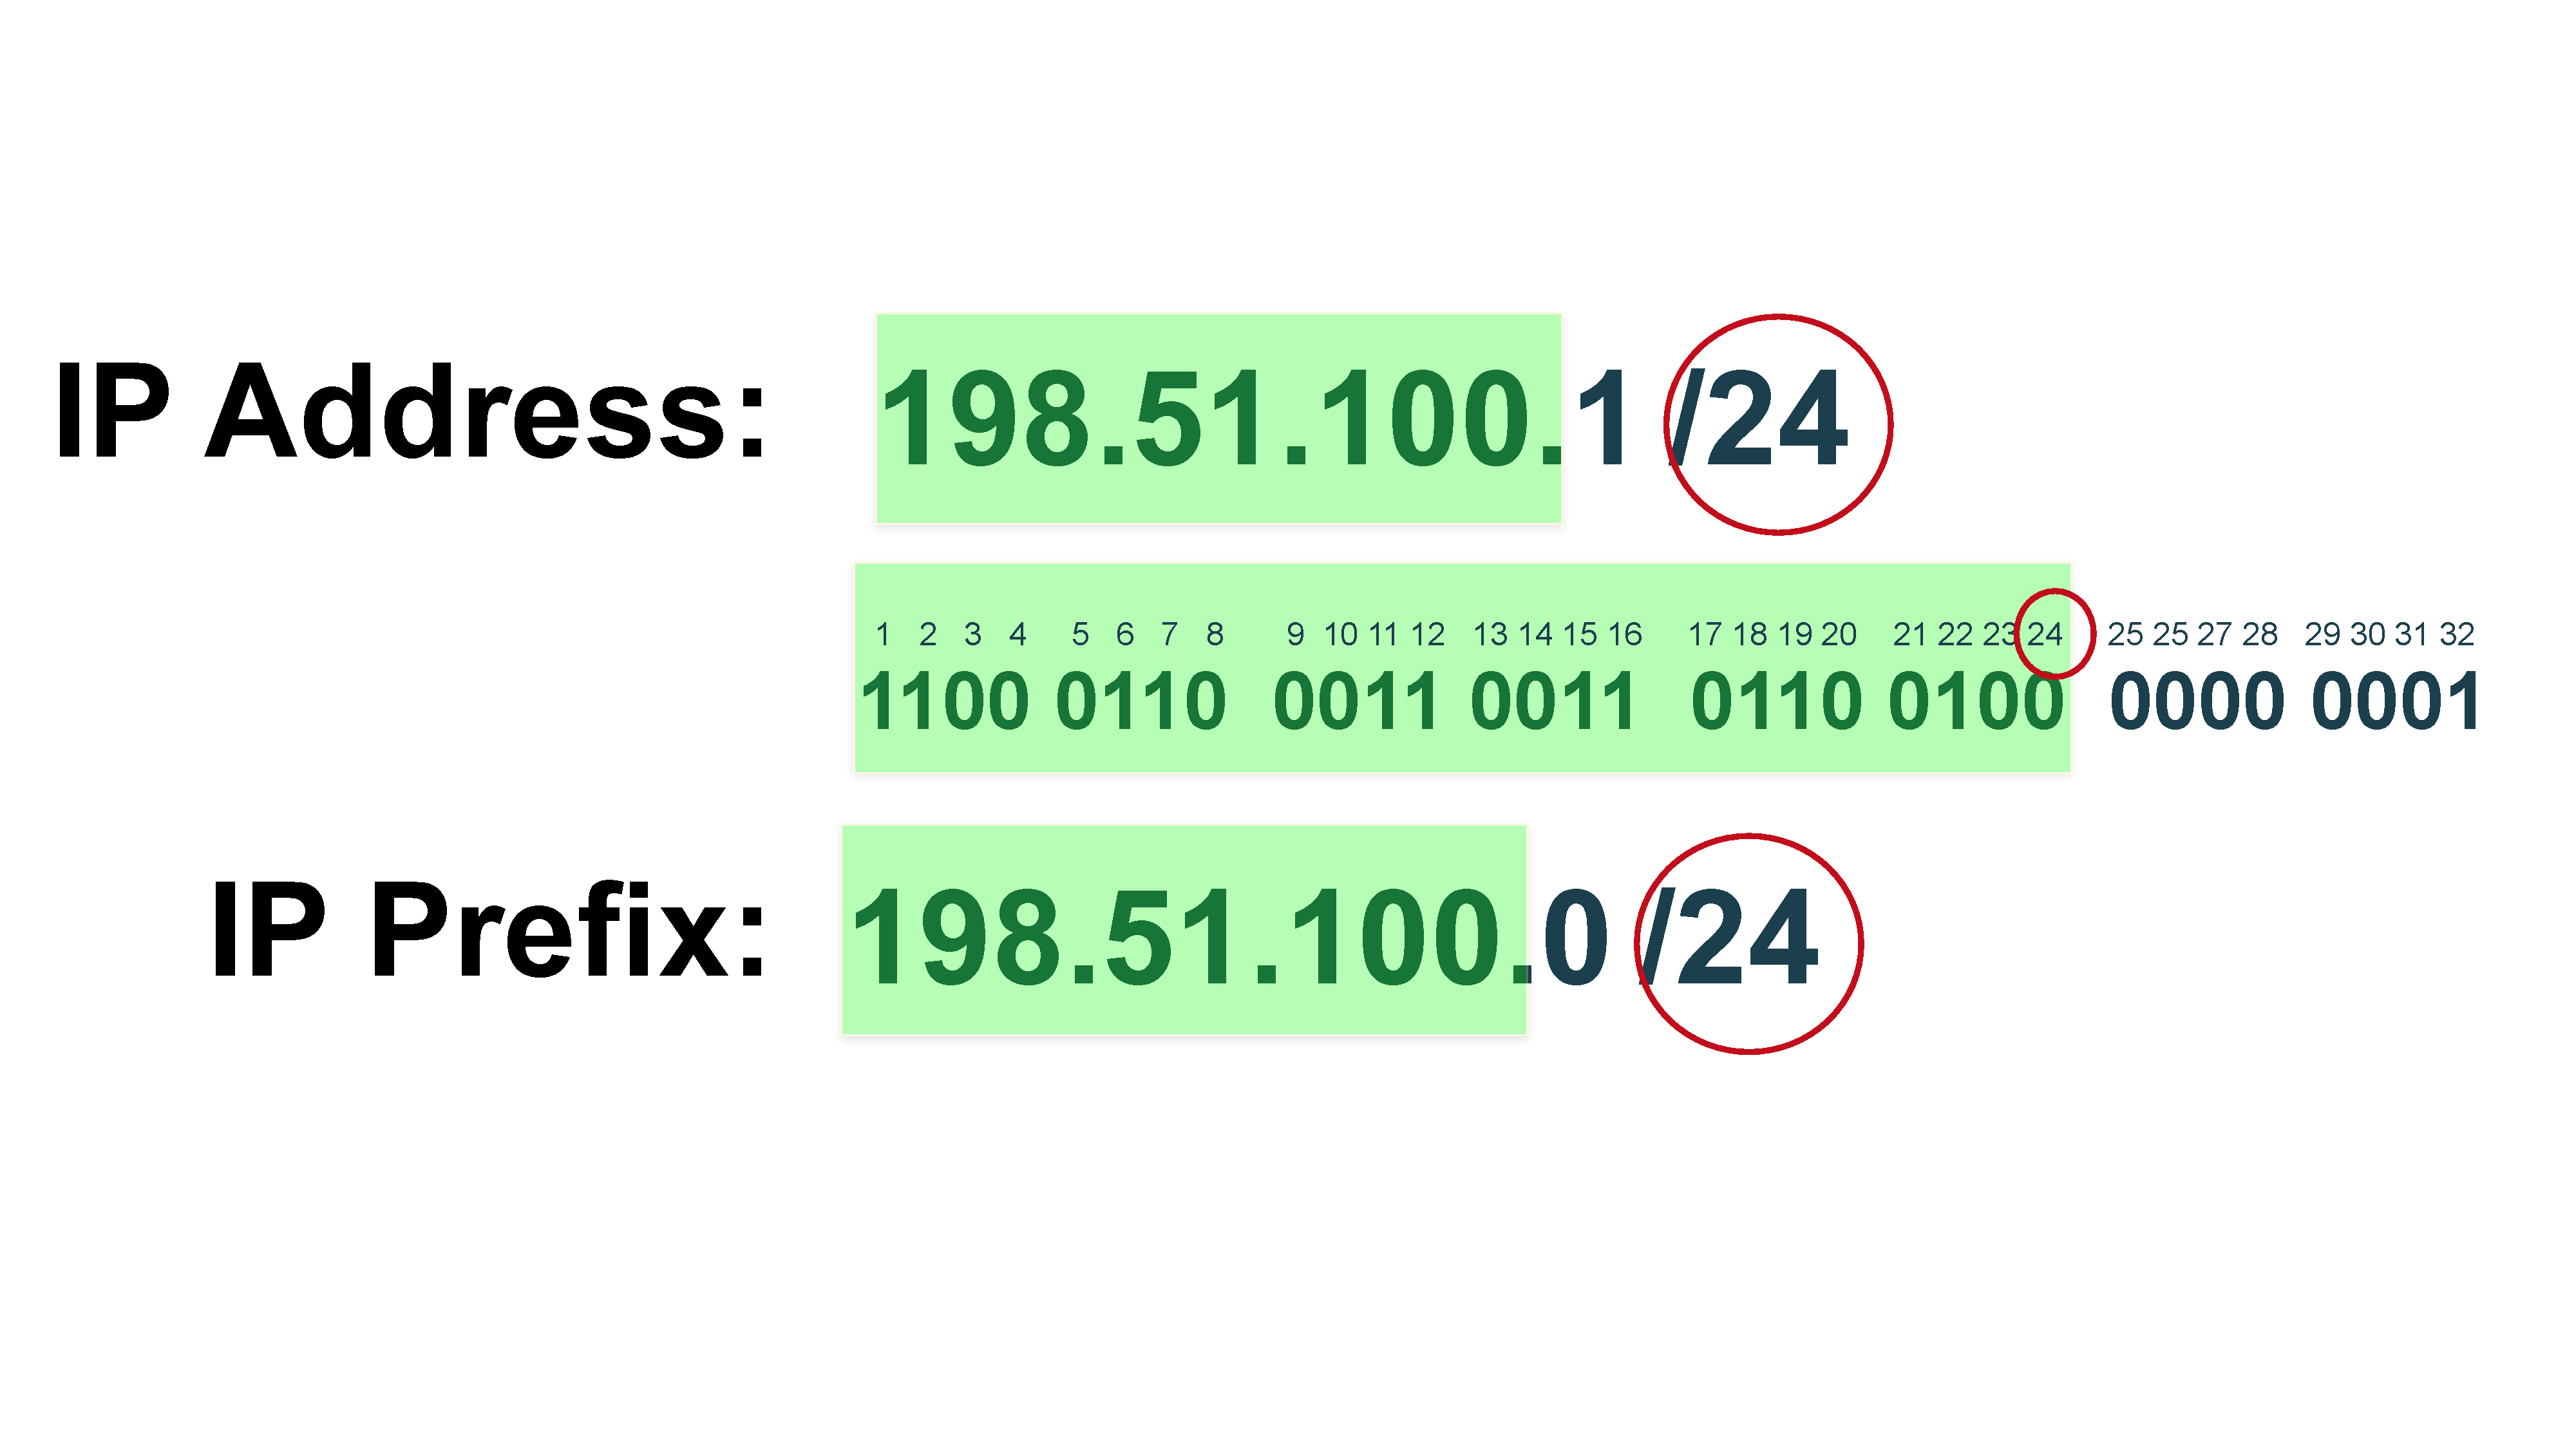
\includegraphics[width=\linewidth,page=1]{img/Drawings.pdf}
  \caption{An IP address and the corresponding IP prefix}
  \label{fig:prefix}
\end{figure}

IPv6 prefixes are similar; they are written as follows: \ip{2001:db8:517::/48}.
Here also the host part is all-zero.

The number behind the `/' is called the prefix length. This is the number of bits
in the network part. The smaller the number, the larger the prefix (larger because
there is more space in the host part of the prefix).

If one prefix is contained in another prefix, you can say that the smaller
prefix (the one with the larger number behind the `/') is \emph{more specific}.

Examples:
\begin{itemize}
  \item \ip{198.51.100.0/26} is more specific than \ip{198.51.100.0/24}.
  \item \ip{2001:db8:6695::/48} is more specific than \ip{2001:db8::/32}.
\end{itemize}

See table~\ref{tab:prefixornot} for some examples of prefixes (and things which are not a prefix).
\begin{table}[hbp]
  \caption{Prefix or not?}
  \label{tab:prefixornot}
  \begin{tabularx}{\textwidth}{lcX}
    \textbf{Item} & \textbf{Prefix?} & \textbf{Explanation} \\
    \hline
    192.168.1.0/24 & Yes & Network part and length \\
    192.168.1.12/24 & No & Host part not zero, this is an IP address and the
                            corresponding netmask \\
    10.0.0.4/30 & Yes & Host part is zero (check!) \\
    80.81.193.0/21 & No & Host part is not zero (convert to binary and check!) \\
    \hline
    2001:db8::/32 & Yes & IPv6 standard prefix \\
    dead:beef:f00d::/48 & Yes & IPv6 is in hexadecimal. So letters a-f are allowed. \\
    2001:db8::4/126 & Yes & Host part is zero. \\
    2001:db8:6695::221:1/96 & No & IPv6 address and netmask. \\
  \end{tabularx}
\end{table}

IPv4 prefixes in the \gls{global routing table} (announced between providers via BGP)
do not come in all sizes. See table \ref{tab:ipv4sizes} for common network sizes. Usually you will not find IPv4 prefixes smaller then /24 in the \gls{global routing table}.
\begin{table}[hbp]
  \caption{Common IPv4 network sizes}
\label{tab:ipv4sizes}
  \begin{tabularx}{\textwidth}{rlrX}
    \textbf{Netmask} & \textbf{Subnet mask} & \textbf{Addresses} & \textbf{Typical use} \\
    \hline
    /8 & 255.0.0.0 & \(2^{24} =\) \tiny{16777216} & Largest block allocated to Internet
        Service Providers (ISPs) or assigned to end users \\
    /9 \ldots /15 \\
    /16 & 255.255.0.0 & 65536 & Large ISP \\
    /17 \ldots /20 \\
    /21 & 255.255.248.0 & 2048 & DE-CIX Frankfurt Peering LAN\\
    /22 & 255.255.252.0 & 1024 & Current allocation of IPv4 space to new ISPs in \gls{RIPE} region \\
    /23 & 255.255.254.0 &  512 \\
    /24 & 255.255.255.0 &  256 & Smallest network routable between providers \\
    /25 & 255.255.255.128 & 128 & \\
    /26 & 255.255.255.192 &  64 & \\
    /27 & 255.255.255.224 &  32 & \\
    /28 & 255.255.255.240 &  16 \\
    /29 & 255.255.255.248 &   8 & Smallest multi-host network (6 hosts)\\
    /30 & 255.255.255.252 &   4 & Often used on point-to-point links (two usable host addresses)\\
    /31 & 255.255.255.254 &   2 & Point-to-point, not possible on all routers\\
    /32 & 255.255.255.255 &   1 & Single host route. Used for loopback interfaces or \gls{blackholing}.\\

  \end{tabularx}
\end{table}

In IPv6 the smallest routable prefix in the \gls{global routing table} is /48. Unlike in IPv4,
when talking about the size of an IPv6 network it is not important how many hosts
an IPv6 network can contain (the standard IPv6 LAN is a /64 and it can
contain
\begin{center}
  \(2^{64} = 18446744073709551616\)
\end{center}
hosts). In IPv6, the question is rather how many /64
sub-networks a network can contain. See table \ref{tab:ipv6sizes} for common IPv6
network sizes.
\begin{table}[hbp]
  \caption{Common IPv6 networks sizes}
  \label{tab:ipv6sizes}
  \begin{tabularx}{\textwidth}{rrXX}
    \textbf{Netmask} & \textbf{Addresses} & \textbf{Used for} & \textbf{Why?}\\
    \hline
    /127 & 2 & Point-to-point \\
    /126 & 4 & Point-to-point \\
    \ldots \\
    /64 & \(2^{64}\) see\footnotemark[1]& LAN & Can address as many
      hosts as you need\\
    \ldots \\
    /56 & \(2^{56}\) & Assigned to residential users & Contains 256 /64 subnets \\
    \ldots \\
    /48 & \(2^{48}\) & Assigned to business users & Contains 65536 /64 subnets \\
    \ldots\\
    /32 & \(2^{32}\) & Current minimum allocation size of IPv6 space to ISPs\\
  \end{tabularx}
\end{table}
\footnotetext[1]{\(2^{24} = 18446744073709551616\)}

\subsection{The Autonomous System}
Another element which needs to be introduced before we can begin with BGP is the
\emph{\gls{Autonomous System}}.

\subsubsection{Motivation}
The Internet is and always has been a ``Network of Networks''. So a big network made up from a lot of small, \emph{independent} networks. Instead of ``independent'' you could also say these part-networks are ``\emph{autonomous}'', so we call them ``\emph{Autonomous Systems}''. And to identify themselves against other part-networks of the Internet, each of them gets an identifier, a so-called \emph{Autonomous System Number}.

\subsubsection{What is an Autonomous System?}
In \cite{rfc1930} an \glsreset{AS}\gls{AS} is defined as follows:
\begin{quotation}
  ``The classic definition of an Autonomous System is a set of routers
      under a single technical administration, using an interior gateway
      protocol (IGP) and common metrics to determine how to route
      packets within the AS, and using an inter-AS routing protocol to
      determine how to route packets to other ASes.''
\end{quotation}

This definition is now replaced by the following more general wording (defined in \cite{rfc1930}):
\begin{quotation}
``An AS is a connected group of one or more IP prefixes run by one
      or more network operators which has a SINGLE and CLEARLY DEFINED
      routing policy.''
\end{quotation}

So the focus is on prefixes and how they are routed:
\begin{itemize}
  \item \emph{\ldots connected\ldots}: An Autonomous System is continuous.
    All entities within are connected with each other.
    \footnote{There are exceptions. AS112 for example is independently operated at multiple locations for DNS reverse resolving of private IP space.}
  \item \emph{\ldots group of one or more IP prefixes\ldots}: This is
    about IP prefixes, not about devices. Routers are not even mentioned.
    All prefixes (or prefix, it can range from one to many) are
    grouped together under an AS and identified by an AS number.
  \item \emph{\ldots run by one or more network operators\ldots}: An AS does
    not have to be run by only one operator if all other conditions
    are matched.
  \item \emph{\ldots SINGLE and CLEARLY DEFINED routing policy\ldots}:
    This is the most important part. Internally and externally all prefixes
    belonging to the same AS are routed the same way. That does not mean
    you cannot adjust the announcement of single prefixes.
\end{itemize}



\subsection{Autonomous System Numbers}
An AS is uniquely identified by an \emph{Autonomous System Number} (ASN). ASNs used to be
16-bit numbers  (defined in \cite{rfc1930}) but some years ago the \gls{IANA} was running out of numbers
to distribute,
so the number space of ASNs has been extended to 32-bit. For this, BGP had to be
extended as well; this was done in \cite{rfc6793}.

Today, AS numbers are 32-bit. You can no longer request a 16-bit number unless
you have a very good reason.

\subsubsection{How to get an AS number}
ASNs are administrated and handed out like IP addresses.
The \gls{IANA} assigns blocks of ASNs to
 \glspl{Regional Internet Registry}; they assign them to \glspl{Local Internet Registry} (= Internet Service Providers), and they hand them out to end users.
To get an AS number you can either:
\begin{itemize}
  \item Become a customer (\gls{Local Internet Registry}) of your local \gls{RIR}, or
  \item ask an existing \gls{Local Internet Registry} to get an ASN for you.
\end{itemize}
The procedures for getting an AS number are different for each region, so please
check online, depending on where you are:
\begin{description}
  \item[Europe, Russia or the Middle East:]
    \url{https://www.ripe.net/publications/docs/ripe-679}
  \item[North Amercia:] \url{https://www.arin.net/resources/request.html#asn}
  \item[South America:] \url{http://www.lacnic.net/1016/2/lacnic/ip-request}
  \item[Asia:] \url{https://www.apnic.net/get-ip/get-ip-addresses-asn/asn-requests/}
  \item[Africa:] \url{https://www.afrinic.net/library/policies/1829-afrinic-consolidated-policy-manual#s7_0}
\end{description}
In general, you must justify your need for an AS number (for example, you want to peer or
have multiple upstream providers).

\subsubsection{Looking up AS numbers}
There are a number of ways you can look up AS numbers.

\paragraph{Whois}
is available on most systems with a command line. Simply type in
\emph{whois AS\emph{nnnn}} and check the output.

\paragraph{PeeringDB}
is an online database of networks who peer. Go to
\url{https://peeringdb.com} and type in the AS number in the search field.

\paragraph{RADB}
mirrors all the databases of the \glspl{RIR}. Just type in the AS number in
the search field.

\paragraph{Regional Internet Registries}
websites can be used also to search for \glspl{ASN}.

\subsection{The AS path}
The AS path is built when announcing prefixes via BGP.
Each AS adds its number to the front of the path. The AS can also be added
multiple times to make an artificially longer AS path. See picture \ref{fig:aspath}
for how an AS path is built by announcing and re-announcing an IP prefix.

\begin{figure}
  \centering
  \includegraphics[width=\linewidth,page=2]{img/Drawings.pdf}
  \caption{How an AS path is built}
  \label{fig:aspath}
\end{figure}


\section{Some theory about routing protocols}
\subsection{Classification of routing protocols}
There are several ways to classify routing protocols:
\begin{itemize}
  \item Static vs. dynamic
  \item Interior protocols vs. exterior protocols
  \item Link state vs. distance vector
\end{itemize}

\subsection{Static vs.\ dynamic routing}
In static routing, you configure all the routing decisions into the routers
statically. So if anything in the network changes, routers have no
way to react and change their routing decisions.

In dynamic routing, routers ``talk'' to each other using a routing protocol
about (for example) the network state and/or reachability of IP addresses. So
in case of a network change, routers can adapt to the new situation.

\subsection{Interior protocols vs.\ exterior protocols}
An \acrfull{IGP} is a protocol which routers under one administrative domain use to communicate with each other about network state and reachability. Examples of \glspl{IGP}
are: \gls{OSPF}, \gls{IS-IS}, \gls{EIGRP}, \gls{RIP}.

Exterior routing protocols are protocols which different administrative entities
use to exchange information. Nowadays, BGP4 is the only exterior protocol
remaining.

\subsection{Link state vs.\ distance vector protocols}
In a link state protocol, each router has a map of the whole network and calculates
the best path to a destination. Examples for link state protocols are OSPF and IS-IS.

In a distance vector protocol, the calculation of the best path is done by routers exchanging
the routing tables with each other and choosing the path with the least number
of hops (or in the instance of BGP:\ number of Autonomous Systems) to cross.

Examples of distance vector protocols are \gls{RIP} and \gls{BGP}.

\section{How a router works}
\begin{figure}
  \centering
  \includegraphics[width=\linewidth,page=10]{img/Drawings.pdf}
  \caption{A simplified diagram of a router}
\label{fig:router}
\end{figure}
But how do these different protocols act together in a router? Please see figure \ref{fig:router} - it shows the various tables in a router and how they interact.

\begin{description}
  \item[Forwarding Table] is often realized in hardware (ASICs). It has to be very fast and is consulted for each and every packet a router forwards. How it works and how it is implemented is different for each router.
  \item[Routing Table] exists for each protocol the router is routing (so most of the time, one table for IPv4 and another table for IPv6). Usually for each prefix the router knows about, it contains one next-hop IP address and the interface via which this IP can be reached.
  \item[Static Routes] are simply installed in the routing table.
  \item[Link State Database] is used by OSPF and contains a complete ``picture'' of the network including all nodes and links in between the nodes. OSPF calculates the best path to a destination and installs it as a route (including a next-hop address) in the routing table.
  \item[BGP Prefix Table] contains all received prefixes from all BGP neighbors. After the BGP process has done its \emph{best prefix selection}, \textbf{one} of these routes is installed in the routing table.
\end{description}

\section{BGP and IPv6}
Usually BGP training programs and manuals have their own chapter about IPv6. But as it is now \DTMfetchyear{heute} and IPv6 should be quite common, all information about how to implement IPv6 routing is directly integrated. You should not setup BGP for IPv4 first and add IPv6 capabilities later - best practice is to integrate IPv6 from the beginning.

BGP is much older then IPv6. The first incarnation of BGP was described in \rfc{1105} in 1989 (building on experience with its predecessor protocol \gls{EGP}) - IPv6 was specified in \rfc{1883} in 1995.

BGP4 (the still-current version) and predecessors were built for distributing IPv4 prefixes only. But unlike IP itself and other routing protocols like \gls{OSPF}, BGP4 was designed with extensibility. So it was not necessary to introduce a new protocol; BGP4 was simply extended.

And because nobody wanted to do this over and over again, the extension to BGP4 was not just to accommodate IPv6, but for multiple network protocols. This was published first in \rfc{2283} (but the most current version of the extensions are in \rfc{4760}). The extension was backward compatible, so routers which had them could communicate with routers which did not have them.

\section{Recommendations}
I rarely give recommendations. This book and the corresponding training seminar should give you the knowledge to make your own choices. However, sometimes perhaps an obvious choice migth not be the best one. In this case you might find my recommendations useful, but wether you follow them or not, is up to you.

Recommendations are clearly marked like this:

\fcolorbox{black}{lgray}{
\begin{minipage}{\linewidth}
\dangersign[8ex] \textbf{Recommendation:}
Read, understand, and make your own choice.
\end{minipage}
}

%!TEX root = ../BGP_for_networks_who_peer.tex
\chapter{Setting up an \gls{IGP}}
\section{Motivation}
\gls{BGP} never runs alone. To distribute the IP addresses of interfaces
within an \gls{AS}, an \glsreset{IGP}\gls{IGP} is needed.

There are several options which \gls{IGP} to use, but normally you will not be free
to choose. Either someone has already made the decision, or you are restricted
on what your router vendor supports.

If you really have several options, keep in mind the following points when
making your decision:
\begin{description}
  \item[Openness:] The IGP must be supported not only by the routers you are using currently, but also by the routers you are purchasing over the next few years.
  \item[IPv6 awareness:] Even if you are currently not using IPv6, you will some time in the future. Your IGP should either support IPv6 or you should be able to run a 2nd IGP in parallel for IPv6.
\end{description}

\section{Configuring OSPF}
\gls{OSPF} runs on top of IP. So you need to configure IP addresses for your
interfaces, and then define the use of OSPF on these IPs. It really helps
if you have all your interface IP addresses out of the same network block
(and use this block for nothing else).

Also, OSPF has the concept of \emph{areas}: You have to define at least one area, called either backbone or area 0 (zero).

Example (Cisco):\label{example-ospf}
\begin{verbatim}
interface GigabitEthernet1/0
 ip address 192.168.2.2 255.255.255.252
!
router ospf 64500
 network 192.168.2.0 0.0.0.255 area 0
\end{verbatim}

This would switch on OSPF on all interfaces with an IP address within 192.168.2.0/24.

Same example for Mikrotik routers:
\begin{verbatim}
/ip address
add address=192.168.2.2/30 interface=ether1 network=192.168.2.0

/routing ospf network
add area=backbone network=192.168.2.0/24
\end{verbatim}

Same example for FRRouting software router:
\begin{verbatim}
interface wlan0.101
  ip address 192.168.2.2/30
!
router ospf
  network 192.168.2.2/30 area 0
\end{verbatim}

On Juniper you enable OSPF on the interfaces:
\begin{verbatim}
  interfaces {
      em0 {
          unit 0 {
              family inet {
                  address 192.168.2.2/30;
              }
          }
      }
  }
  protocols {
    ospf {
      area 0.0.0.0 {
        interface em0.0;
      }
    }
  }
\end{verbatim}

Keep in mind that OSPFv2 (the ``standard'' OSPF version) supports IPv4 only. This is completely fine; for IPv6 you can use OSPFv3 to keep things separate. Or you can run IS-IS which supports IPv4 and IPv6.

\section{Configuring IS-IS}
\gls{IS-IS} does not run on top of IP but runs directly on layer 2 (Ethernet or other). So you do not have to define the network it runs on, but the interfaces you want it enabled on.

\emph{Important}: The protocols you enable it for must be the same on both sides of a connection. So if you enable IS-IS for IPv4 and IPv6 on one interface, you must do so as well on the connected interface.

Example for IS-IS on Cisco:
\begin{verbatim}
interface GigabitEthernet0/0
  ip address 192.168.2.2 255.255.255.252
  ipv6 address autoconfig
  ip router isis
  ipv6 router isis
!
router isis
  net 49.0000.0000.0000.0001.00
\end{verbatim}
The number behind the ``net'' statement is the router-id and must be unique within your network.

Mikrotik does not support IS-IS.

Example for IS-IS on FRRouting:
\begin{verbatim}
router isis myname
  net 49.0000.0000.0000.0001.00
!
interface eth1
  ip address 192.168.2.2/30
  ipv6 address autoconfig
  ip router isis myname
  ipv6 router isis myname
\end{verbatim}

Example for IS-IS on Juniper is a little bit more complex. For the loopback interface \emph{lo0} we configure a static IPv6 address, for the ethernet interface we use auto-configuration. Also, the router-id goes into the loopback interface and \emph{family iso} has to be enabled on all interfaces where IS-IS is to be used.
\begin{verbatim}
  interfaces {
      em0 {
          unit 0 {
              family inet {
                  address 192.168.2.2/30;
              }
              family iso;
              family inet6;
          }
      }
      lo0 {
          unit 0 {
              family inet {
                  address 192.168.1.3/32;
              }
              family inet6 {
                address 2001:db8:500::1:3/128;
              }
              family iso {
                  address 49.0000.0000.0000.0003.00;
              }
          }
      }
  }
  protocols {
    isis {
        interface em0.0;
        interface lo0.0;
    }
\end{verbatim}


\section{Configuring OSPFv3}
To integrate IPv6 a new version of OSPF was necessary - this came into being as OSPFv3. Except for virtual links, OSPFv3 uses IPv6 link-local addressing. It is configured on the interface, not on a network like OSPFv2.

The only remains of 32bits are area and router ids - they are still 32bit like IPv4 addresses.

Example for OSPFv3 on Cisco IOS:
\begin{verbatim}
interface Loopback0
  ipv6 address 2001:DB8:500::1:3/128
  ipv6 ospf 64500 area 0
!
interface GigabitEthernet0/0
  ipv6 address autoconfig
  ipv6 ospf 64500 area 0
\end{verbatim}
In this example, \emph{64500} is the process id of the OSPFv3 process - you can choose any number. It is not even necessary to define the process itself - simply enable OSPv3 on all interfaces where you want to use it. Whether you want to use auto-configured IPv6 addresses on your link interfaces or static IPv6 addresses is up to you.

Example for Mikrotik:
\begin{verbatim}
/ipv6 address
  add address=2001:DB8:500::1:1/128 interface=loopback0
  add interface=ether0 address=2001:DB8:496::1:2/126

/routing ospf-v3 interface
  add area=backbone interface=loopback0
  add area=backbone interface=ether0
\end{verbatim}

Example for FRRouting:
\begin{verbatim}
router ospf6
  router-id 192.168.1.1
  interface dummy0 area 0.0.0.0
  interface eth1 area 0.0.0.0
  interface eth2 area 0.0.0.0
\end{verbatim}
You have to configure an (IPv4-like) router-id manually - the best approach is to use the IPv4 address of your Loopback interface. Also the area notation is written like an IPv4 address.

Example for Juniper:
\begin{verbatim}
  protocols {
    ospf3 {
        area 0.0.0.0 {
            interface lo0.0;
            interface em0.0;
        }
    }
  }
\end{verbatim}

\iffalse % ---------------- do not print ----------------------

\section{Experiment 1a, 1b and 1c: Setup IGP}
Please see separate experiment documentation.

\section{Experiment \theexperiment}
\subsection{Network Setup}
Network is a ring-shaped network out of all participants' routers (see
picture \ref{fig:exp1}).

\begin{figure}
  \includegraphics[width=\linewidth]{img/i-wt-BGP-Raspi-Experiment01-iBGP-01.png}
  \caption{Experiment 1 - Setting up an IGP}
  \label{fig:exp1}
\end{figure}

\subsection{Task}
To complete this experiment, you must:
\begin{itemize}
  \item Configure your assigned loopback IP address on your router
  \item Configure \gls{OSPF} on your router so it talks to its neighbors
  \item Redistribute your loopback address via OSPF. Use
  \begin{verbatim}
    redistribute connected subnets
  \end{verbatim}
  for this.
  \item See the other routers loopback addresses in your routing table.
\end{itemize}

\fi % ------------------------------------

%!TEX root = ../BGP_for_networks_who_peer.tex
\chapter{iBGP - BGP within one Autonomous System}
\section{What is iBGP?}
iBGP is not a separate protocol. It is simply the ``flavor'' of BGP which is spoken between routers which are in the same \glsreset{AS}\gls{AS}.

All BGP routers use \gls{TCP} to communicate with each other.

Prefixes are distributed in iBGP according to the following rules:
\begin{itemize}
  \item Each router only distributes the best route for a prefix
  \item Prefixes received via iBGP (from the same \gls{AS}) are \emph{not} distributed
  \item Prefixes received via eBGP (from other \glspl{AS}) are distributed.
\end{itemize}
Since prefixes received from routers via iBGP are not redistributed (there are exceptions, see \ref{routereflector}), iBGP has to be \emph{fully meshed}, meaning that each router needs to have an iBGP session to all other routers.

By default, the next-hop address of a prefix received via eBGP is redistributed \emph{unchanged}. If you do not want to redistribute the IP addresses (IPv4 and IPv6) of external interfaces within your \gls{AS}, you need to set an option on your iBGP sessions to change this next-hop address to the address of your iBGP session. Usually this option is named \emph{next-hop-self}.

BGP4 is multi-protocol capable. That means that you can use IPv4 to both distribute IPv4 and IPv6 prefixes. However, this is not really advisable, as the next-hop address (which is also distributed) has to be set manually then. Best practice is to use IPv4 transport to distribute IPv4 prefixes and IPv6 transport to distribute IPv6 prefixes.

\section{Configuring iBGP}
Like stated above, iBGP uses \gls{TCP} to communicate. So to set up an iBGP session between two routers, you need to define:
\begin{itemize}
  \item IP address to connect to
  \item local IP address to be used as source (optional, but recommended)
\end{itemize}

\subsection{About the Loopback interface}
If you do not tell BGP which local IP address to use, routers use as source IP the IP address of that interface on which packets leave the router. This might not be advisable, because if that interface goes down all iBGP sessions using the IP address of this interface get disrupted, even if there is another path to the remote router.

\begin{figure}
  \centering
  \includegraphics[width=\linewidth,page=11]{img/Drawings.pdf}
  \caption{iBGP connection with and without Loopback interface}
  \label{fig:ibgploopback}
\end{figure}

Therefore, best practice is to define a \emph{Loopback interface}, an artificial internal interface which is not connected to anything and always stays up. As the Loopback interface is not connected to anything, the address of the Loopback interface should be a /32 in IPv4 and a /128 in IPv6.

This is illustrated in figure \ref{fig:ibgploopback} - if an interface IP is used, the TCP connection gets disrupted in the instance of a circuit failure and has to be re-established (of course the iBGP connection also has to be re-established, including the exchange of all BGP prefix information). If a Loopback interface is used, the TCP connection is simply re-routed and the iBGP connection will stay up.

Also, for IPv6 you can easily use link-local addresses on the interconnect and just have the Loopback statically configured and use it for iBGP. If you have the luxury to choose, you might have ``similar looking'' IPv4 and IPv6 addresses for the Loopback interface. But beware of giving your IPv6 addresses any ``meaning'' - just select an IPv6 prefix and assign addresses out of it. Otherwise, you will run into problems later on, as giving meaning to addresses seldom scales.

\subsection{Lifecycle of a BGP connection}
If you configure BGP on a router, if the session comes up, everything is fine. But sometimes the session cannot be established, and if you check the BGP session table you might see a ``status'' of the session. Some of these states that a session can be in are self-explanatory, but some require more explanation. You will find below a list of session states you might see. These session states are defined in \rfc{4271} as a finite state machine. All states described are \emph{per peer}.

\begin{figure}
  \centering
  \includegraphics[width=\linewidth,page=15]{img/Drawings.pdf}
  \caption{BGP finite state machine}
  \label{fig:bgpfsm}
\end{figure}

\begin{description}
  \item[Idle] is the initial state of any BGP connection. In this state, no resources are allocated to the session and incoming connection attempts are refused. Depending on events, the state is either changed to \emph{active} or \emph{connect}.
  \item[Connect] means that BGP is waiting for a TCP connection to a neighbor to be completed. If this succeeds, the state of the session is changed to \emph{OpenSent}, if not, it's either back to \emph{idle} or to \emph{active}.
  \item[Active] - you will see this state a lot. Be aware that it means that a BGP session is \emph{not} established. BGP in this state waits for an incoming TCP connection. If the retry timer expires, the state changes to \emph{connect} to re-try connecting.
  \item[OpenSent] - BGP has established a TCP connection, sent an \emph{open} message to the peer and waits for an incoming \emph{open} message. Once received and checked ok, the state is changed to \emph{OpenConfirm}. In case of a timeout or an error, the state falls back to either \emph{idle} or \emph{active}.
  \item[OpenConfirm] - here BGP waits for a \emph{keepalive} or \emph{notification} message from the peer. We are nearly there! If one of these messages are received, the state is changed to \emph{established}. If something goes wrong, again we fall back to either \emph{idle} or \emph{active}.
  \item[Established] is the state that you want your BGP session to be in. Prefixes can be exchanged and everything is fine. From here you can only go back to \emph{idle}.
\end{description}
See also figure \ref{fig:bgpfsm} for the states and how they may change.

\subsubsection{Notifications on shutdown}
When a BGP session is shut down, the party initiating the cease of the BGP session is sending out a notification. \rfc{4486} lists a number of pre-defined reasons for shutting down a session.
\begin{description}
  \item[Maximum number of prefixes reached] - this means that the other side is sending more prefixes then the receiver allows (see \ref{maxprefix}). Sending of this notification is mandatory.
  \item[Administrative shutdown] - the session has been shut down using a configuration command.
  \item[Peer de-configured] -  the BGP session has been de-configured.
  \item[Administrative reset] - the session has been reset using a command. It will be re-established again.
  \item[Connection rejected] - if the BGP session is disallowed \emph{after} a TCP session has already been established this notification should be sent.
  \item[Other configuration change] - if a session is reset for any other reason as the ones stated above.
  \item[Connection collision resolution] - this should be sent if a collision occurs  while establishing a session.
  \item[Out of resources] - this may be sent if a router runs out of resources (like memory) and tears down the session.
\end{description}

The newer \rfc{8203} enhances the \emph{Administrative Reset} and \emph{Administrative Shutdown} reasons with the possibility for the shutting down party to add a free-form text message.

It is up to the receiver of all these notifications to do something with them (or not) - for example the DE-CIX route server displays them in the looking glass - see \url{https://lg.de-cix.net}.

\subsubsection{Timers}
To keep BGP sessions alive (well, more to check \emph{if} they are still alive) BGP speakers send each other \emph{keepalive} messages. The following timers  exist:
\begin{description}
  \item[Keepalive Timer:] This timer takes care of sending \emph{keepalive} messages to the BGP neighbor. Everytime it expires a keepalive message is sent and the timer is reset (it is also reset every time a normal update message is sent). The start value of the Keepalive Timer may be configurable, it is usually one third of the Hold Timer.
  \item[Hold Timer:] This timer determines how long a BGP session is considered being open without a \emph{keepalive} or update message received. The start value of the timer is negotiated during session setup - it is usually three times of the initial value of the \emph{Keepalive Timer}. It can be configured on a per-neighbor basis and in session initiation the lowest value configured of the two peers wins. A usual default value is 180 seconds. It is not a good idea to set this timer too aggressively short - this would increase the CPU load of the BGP process.

  If the hold timer expires, the BGP session is considered being down and all prefixes received from this session are removed from the BGP table and the session state is set to \emph{idle}.
\end{description}

Given the usual default values it may take up to three minutes to detect if a BGP neighbor is down. During that time, if the interface the session is established on is still up, prefixes received via this session are still valid and so traffic may be dropped.

% For a faster detection if a neighbor is down today usually \gls{BFD} is used.

\fcolorbox{black}{lgray}{
\begin{minipage}{\linewidth}
\dangersign[8ex] \textbf{Recommendation:}
Do not modify the BGP timers unless you are absolutely sure you know what you are doing. If you want to take down BGP sessions fast if a neighbor goes down, use \gls{BFD}
\end{minipage}
}



\subsection{Fully Meshed vs. Route Reflector}
\label{routereflector}
As an iBGP speaker by default does not forward prefixes received via iBGP, your iBGP nodes need to be \emph{fully meshed}. This means each BGP speaking router needs an iBGP connection to any other BGP speaking router (with $n$ routers, each router therefore has $(n-1)$ iBGP sessions; in your network you have $n*(n-1)/2$ iBGP sessions in total).

\begin{figure}
  \centering
  \includegraphics[width=\linewidth,page=12]{img/Drawings.pdf}
  \caption{Application of a Route Reflector}
  \label{fig:routereflector}
\end{figure}

Now imagine one of your edge routers is connected in a non-redundant way to the rest of your network (see figure \ref{fig:routereflector}). There is no point setting up multiple iBGP sessions - if the connection to this edge router fails, \emph{all} of them will go down. This is a good application for using a \emph{Route Reflector}. A \gls{Route Reflector} sends out all prefixes (even those received via iBGP) to its \glspl{Route Reflector Client}. These clients usually have only one BGP connection - to their server.

Using route reflection, it is also possible to build iBGP networks using only Route Reflectors and clients. These architectures are beyond the scope of this document.

Configuration has only to be done on the reflector side; usually it's just one statement.
\begin{description}
  \item[Cisco:] \begin{verbatim}
    neighbor 172.16.1.2 route-reflector-client
    neighbor 172.16.1.2 next-hop-self all
\end{verbatim}
  ``next-hop-self all'' sets the next hop of announced prefixes to the IP of the reflector for all prefixes announced to the client. With this set, you might not even have to run an \gls{IGP} on your client.
  \item[Mikrotik:] \begin{verbatim}
  /routing bgp peer
  add name=R2 nexthop-choice=force-self \
    remote-address=172.16.1.2 \
    remote-as=64500 route-reflect=yes
\end{verbatim}
The ``force-self'' in nexthop-choice sets the interface IP of the reflector as nexthop when announcing prefixes to the client.
  \item[Juniper:] To configure a route reflector you simply have to give it a \emph{cluster} id, best is to do that in a group: \begin{verbatim}
  protocols {
      bgp {
          local-as 64500;
          group internal-rr {
              type internal;
              family inet {
                  unicast;
              }
              export rr-next-hop;
              cluster 172.16.1.1;
              peer-as 64500;
              neighbor 172.16.1.2;
          }
      }
  }
\end{verbatim}
Setting the next hop is done with a policy-statement: \begin{verbatim}
policy-options {
  policy-statement rr-next-hop {
      term 1 {
          from protocol bgp;
          then {
              next-hop self;
          }
      }
  }
}
\end{verbatim}
\end{description}

In this case, using a Loopback interface for the session and for next-hop is not advisable. The client is not connected redundantly, so if the connection goes down a Loopback interface does not help. Also, when using the interface IP for the iBGP session \emph{and} a forced next-hop for announced prefixes, you do not even have to run an \gls{IGP} to the client.

\subsection{Keeping the configuration short}
In general, it is advisable to keep the iBGP configuration as short as possible. Depending on the router you are using, there is the possibility to group BGP commands. On Cisco this is called a ``peer group''.

To keep IPv4 and IPv6 configuration separate, use one peer group for each - also most routers do not allow mixing of configuration here.

\subsection{Cisco example}
Configuration example for Loopback interface and iBGP for Cisco IOS:
\begin{verbatim}
  interface Loopback0
    ip address 172.16.1.1 255.255.255.255
    ipv6 address 2001:db8:500::1:1/128
  !
  router bgp 64500
    neighbor internal peer-group
    neighbor internal remote-as 64500
    neighbor internal update-source Loopback0
    !
    neighbor internal6 peer-group
    neighbor internal6 remote-as 64500
    neighbor internal6 update-source Loopback0
    !
    neighbor 172.16.1.2 peer-group internal
    neighbor 172.16.1.3 peer-group internal
    neighbor 172.16.1.4 peer-group internal
    !
    neighbor 2001:db8:500::1:2 peer-group internal6
    neighbor 2001:db8:500::1:3 peer-group internal6
    neighbor 2001:db8:500::1:4 peer-group internal6
    !
    address-family ipv4
      neighbor internal next-hop-self
    !
    address-family ipv6
      neighbor internal6 next-hop-self
    ...
\end{verbatim}
This is the minimum configuration. The local AS number is specified in the router command and the remote AS in the peer group.

The ``next-hop-self'' command ensures that prefixes received from other ASes  get this router's IP set as next-hop address (so external IPs do not have to be redistributed using our IGP). Note that this is below the ``address-family'' statement.

To set up iBGP sessions to each remote router, you need only configure its IP address and that it belongs to the peer group ``internal''.

To distribute the IP address of the Loopback interface, we extend the configuration of our IGP as shown in \ref{example-ospf}:
\begin{verbatim}
  router ospf 64500
    network 192.168.2.0 0.0.0.255 area 0
    redistribute connected subnets
\end{verbatim}
So again: We set up iBGP sessions between the Loopback interfaces of all routers.

For IPv6, if you use IS-IS, simply enable it on the Loopback interface:
\begin{verbatim}
  interface Loopback0
    ip router isis
    ipv6 router isis
\end{verbatim}

Similarly for OSPFv3; here you also have to add the number of the OSPFv3 process and an area:
\begin{verbatim}
  interface Loopback0
    ipv6 ospf 64500 area 0
\end{verbatim}

\subsection{Mikrotik example}
Mikrotik does not directly support Loopback interfaces, but you can use an empty bridge interface instead:
\begin{verbatim}
  /interface bridge
  add name=loopback0
  /ip address
  add address=172.16.1.1/32 interface=loopback0 network=172.16.1.1
  /ipv6 address
  add address=2001:DB8:500::1:1/128 interface=loopback0
\end{verbatim}

As an \gls{IGP}, Mikrotik only supports OSPFV2 and OSPFv3:
\begin{verbatim}
  /routing ospf-v3 interface
  add area=backbone interface=loopback0
  add area=backbone interface=ether1
  add area=backbone interface=ether2
  ...
\end{verbatim}

Also, Mikrotik does not support peer groups; you have to configure everything in the peer entry:
\begin{verbatim}
  /routing bgp instance
  set default as=64500 router-id=172.16.1.1

  /routing bgp peer
  add name=R2 nexthop-choice=force-self remote-address=172.16.1.2 remote-as=\
    64500 update-source=loopback0
  add name=R3 nexthop-choice=force-self remote-address=172.16.1.3 remote-as=\
    64500 update-source=loopback0
  add name=R2-6 nexthop-choice=force-self remote-address=2001:db8:500::1:2 \
    remote-as=64500 address-families=ipv6
  add name=R3-6 nexthop-choice=force-self remote-address=2001:db8:500::1:3 \
    remote-as=64500 address-families=ipv6
\end{verbatim}

We restrict the IPv6 iBGP sessions to IPv6, using the ``address-families'' statement. Otherwise the IPv6 sessions would want to announce IPv4 prefixes as well, and we decided to keep this separate. On the IPv4 sessions, the address-families config is not required, as IPv4 is distributed by default.

Also keep in mind that on both sides of an iBGP (or any BGP) session, the same address families must be configured - otherwise the session does not come up.

% \subsection{Juniper Example}

%!TEX root = ../BGP_for_networks_who_peer.tex
\chapter{eBGP - Connecting to the outside world}
\label{ch:eBGP}
\section{What is eBGP?}
We call a BGP session an eBGP (external BGP) session if it connects to a different Autonomous System.

\subsection{Differences between iBGP and eBGP}
There are a couple of differences between the two flavors of BGP.

One difference is that, while in iBGP it does not matter how many ``hops'' (in terms of the IP protocol) a neighbor is away, in eBGP the neighbor usually is directly connected.  You can change this behavior if you configure the neighbor as being a ``multi-hop'' neighbor (\texttt{neighbor x.x.x.x ebgp-multihop}).

\fcolorbox{black}{lgray}{
\begin{minipage}{\linewidth}
   How does it work that eBGP packets only travel to the next adjacent node?
   The answer lies with the IP \emph{TTL (Time to Live)} counter: The sender sets the counter to one, so packets get discarded if the eBGP neighbor is more then one hop away. See chapter~\ref{ch:security} to learn about a more secure approach to this.
\end{minipage}
}

Also the next-hop of IP addresses received via eBGP is set to the address the sender of the prefixes (your eBGP neighbor) specified. If you forward this prefix then via iBGP, this next hop is either unchanged or set to the IP of your router (\texttt{neighbor x.x.x.x next-hop-self}).

The router receiving a prefix via eBGP also checks if the next-hop IP address is accessible via the interface the prefix is received. If it is not, the eBGP announcement is discarded.

Your router also checks the AS-Path of all received prefixes. If your own AS number is in that path, the prefix is also discarded (this can be switched off by a config command which is \emph{not recommended}).

Other measures to ignore unwanted prefixes etc. have to be configured manually using filter lists or route-maps. More about this you can read in chapter~\ref{ch:security}.


\subsection{Best practices}
It is best practice to not let prefixes in from outside without some filtering. Most of this filtering will be covered in chapter~\ref{ch:security} when we talk about BGP security. At this time we will define empty filters for sending and receiving prefixes (named ``-out'' for sending ``-in'' for receiving). We will extend these filters later.

If your router supports it, it's again best practice to define a peer-group and have all common configuration in the peer-group (you need two peer-groups again, one for IPv4 and one for IPv6).

It is strongly recommended that you setup a filter to \emph{not announce any} prefixes initially when setting up a completely new eBGP peer group. We will do so by configuring our ``-out'' route-map to deny everything.

Depending on your routers BGP implementation, configuration commands become active the moment you hit the ``enter'' key. So if you configure an eBGP neighbor \emph{without} any filtering and the neighbor already has configure its side, you start flooding your complete BGP table immediately. \rfc{8212} addresses this problem by requesting that eBGP sessions without any \emph{configured} filtering get an automatic \emph{deny-all} filter by default. Some vendors have already implemented this, some made it optional.

Some routers allow  received information (before filter processing) to be stored in a separate table (at the cost of increased memory usage). To debug your filters, this is very useful, so I suggest you turn it on (see examples below).

\subsection{Sources and destinations of prefixes}
\begin{figure}
  \centering
  \includegraphics[width=\linewidth,page=17]{img/Drawings.pdf}
  \caption{eBGP Roles}
  \label{fig:bgproles}
\end{figure}

If you look at possible BGP neighbors, you come up with some categories you receive prefixes from and announce prefixes to. \rfc{9234} defines to following BGP neighbor roles and relationships:
\begin{description}
  \item[Provider, Customer:] A provider announces all known prefixes to a customer, a customer announces only its own and its customers prefixes to a provider.
  \item[Peer, Peer:] They announce their own and their customers prefixes to each other.
  \item[Route Server, Route Server Client:] Similar to peers, a route server announces all prefixes to a route server client, which announces their own and their customers prefixes to a route server.     
\end{description}
See picture~\ref{fig:bgproles} for a graphical expression of roles and relationships.
These relationships must be expressed in filter configurations. You can do that manually (better: automated) with allow-lists or you can implement sophisticated mechanisms. Choose what ever fits best to your network size. Chapter~\ref{ch:security} and chapter~\ref{ch:BGP Communities} will give you some ideas.

\subsection{Cisco example}
In this simple example we \emph{deny} any outgoing prefixes.
\begin{verbatim}
  route-map upstream-out deny 10
  !
  route-map upstream-in permit 10
  !
  route-map upstream6-out deny 10
  !
  route-map upstream6-in permit 10
  !
  router bgp 64500
    neigbor upstream peer-group
    neigbor upstream6 peer-group
    neighbor 192.168.3.2 remote-as 65550
    neighbor 192.168.3.2 peer-group upstream
    neighbor 2001:db8:300::2 remote-as 65550
    neighbor 2001:db8:300::2 peer-group upstream6
    !
    address-family ipv4
      neigbor upstream route-map upstream-in in
      neigbor upstream route-map upstream-out out
      neigbor upstream soft-reconfiguration inbound
      neigbor upstream6 route-map upstream6-in in
      neigbor upstream6 route-map upstream6-out out
      neigbor upstream6 soft-reconfiguration inbound
      neighbor 192.168.3.2 activate
      no neighbor 2001:db8:300::2 activate
    !
    address-family ipv6
      neigbor upstream route-map upstream-in in
      neigbor upstream route-map upstream-out out
      neigbor upstream soft-reconfiguration inbound
      neigbor upstream6 route-map upstream6-in in
      neigbor upstream6 route-map upstream6-out out
      neigbor upstream6 soft-reconfiguration inbound
      no neighbor 192.168.3.2 activate
      neighbor 2001:db8:300::2 activate
\end{verbatim}
The \emph{soft-reconfiguration inbound} ensures that you can check what your router receives before it is processed by the incoming route-map.

Take note of how the address-family parts and entry act together. ``address-family'' relates to the \emph{announced} prefixes; the IP address of the neighbor defines the protocol of the BGP session. With the ``activate'' clauses we switch off IPv4 prefix announcement on the IPv6 sessions and switch on IPv6 announcement. On the IPv4 sessions, we do it the other way around. What increases the confusion is that some of these statements are considered to be default at Cisco and therefore are omitted in the config.

Do we need different route-maps for IPv4 and IPv6? That's dependent on their complexity. \emph{If} you want to do any IP related filtering (ip address lists, prefix lists) having two (or four) route-maps is recommended.

\subsection{Mikrotik example}
\begin{verbatim}
  /routing bgp instance
  set default as=64500 router-id=192.168.1.1

  /routing bgp peer
  add name=upstream-AS65550 in-filter=upstream-in \
    out-filter=upstream-out \
    remote-address=192.168.3.2 remote-as=65550
  add name=upstream6-AS65550 in-filter=upstream6-in \
      out-filter=upstream6-out \
      remote-address=2001:db8:300::2 remote-as=65550 \
      address-families=ipv6

  /routing filter
  add chain=upstream-in action=accept
  add chain=upstream-out action=discard
  add chain=upstream6-in action=accept
  add chain=upstream6-out action=discard
\end{verbatim}
Mikrotik does not support peer-groups or similar, so everything needs to be configured on every peer. Here the ``address-families'' parameters determines what kind of prefixes are announced and accepted. Again, the default ``IPv4 only'' can be omitted - making the configuration rather more then less confusing.

We also do not announce any prefixes here (by using the \emph{action=discard} statement in our filters).

\subsection{FRRouting example}
In FRRouting we can put the \emph{activate} clauses into the peer group, also we enable \rfc{8212} automatic filtering:
\begin{verbatim}
route-map upstream-out deny 10
!
route-map upstream-in permit 10
!
route-map upstream6-out deny 10
!
route-map upstream6-in permit 10
!
router bgp 64500
  bgp ebgp-requires-policy
  neigbor upstream peer-group
  neigbor upstream6 peer-group
  neighbor 192.168.3.2 remote-as 65550
  neighbor 192.168.3.2 peer-group upstream
  neighbor 2001:db8:300::2 remote-as 65550
  neighbor 2001:db8:300::2 peer-group upstream6
  !
  address-family ipv4
    neigbor upstream route-map upstream-in in
    neigbor upstream route-map upstream-out out
    neigbor upstream soft-reconfiguration inbound
    neighbor upstream activate
    neigbor upstream6 route-map upstream6-in in
    neigbor upstream6 route-map upstream6-out out
    neigbor upstream6 soft-reconfiguration inbound
    no neighbor upstream6 activate
  exit-address-family
  !
  address-family ipv6
    neigbor upstream route-map upstream-in in
    neigbor upstream route-map upstream-out out
    neigbor upstream soft-reconfiguration inbound
    neigbor upstream6 route-map upstream6-in in
    neigbor upstream6 route-map upstream6-out out
    neigbor upstream6 soft-reconfiguration inbound
    no neighbor upstream activate
    neighbor upstream6 activate
  exit-address-family
\end{verbatim}
% \subsection{Juniper example}

%!TEX root = ../BGP_for_networks_who_peer.tex
\chapter{Becoming multi-homed}
\section{What is being multi-homed (in terms of BGP)?}
In the last chapter, we set up eBGP to one ``upstream'' provider. But in practice, this is not what we want - we would be dependent on only one connection to the outside world and would be offline if it failed (which is exactly the same as running no BGP at all).

So we need to connect to (at least) one more upstream. And to make our network even more resilient and to drive down cost, we will also connect to an Internet Exchange and set up peering sessions there.

This increases our network (and BGP) complexity somewhat, but if we plan (and configure) carefully, then this complexity is easily manageable. The purpose of this chapter is to offer you best practices, so that you do not run into an over-complex network set-up later on.

\section{What changes when you become multi-homed?}
When you have only one connection to the outside, your world is simple:
\begin{itemize}
  \item You either have a default route to your upstream and send everything which is not inside your own network to there, or
  \item you get a full routing table from your upstream, but still have only one connection to the outside to send traffic to.
\end{itemize}

With two (or more) connections to the outside, it gets more interesting:
\begin{itemize}
  \item You receive the same prefix(es) via BGP from provider A and provider B; which one do you prefer?
  \item What criteria does BGP use per default to decide which prefix announcement is ``better''?
  \item Can you influence or override this decision? (yes, you can)
  \item When to influence best prefix selection (this is what this is called) and when to leave it to the defaults? (this is lifelong learning).
\end{itemize}

\section{Configuring multi-homing}
\subsection{Network setup}
\begin{figure}
  \centering
  \includegraphics[width=\linewidth,page=3]{img/Drawings.pdf}
  \caption{Example setup with two upstream providers and peering}
  \label{fig:multihoming}
\end{figure}
See figure \ref{fig:multihoming} for our example network. Your AS64500 is connected two upstreams AS64496 and AS65550. Behind them we have a couple of ASes for distributing prefixes - their AS numbers are not really important. One of them also peers with you.

\subsection{Receiving prefixes}
For our somewhat simplified view of the Internet, we receive a handful of prefixes originated by AS517 over various paths.
\iffalse
Configure your router according to the experiment sheet and have a look at your BGP table to see which prefixes are considered ``best''.
\fi

\subsection{Sending prefixes}
You should always only send your own prefixes and those of your customers. Beware - if you do not configure any filtering, your router sends out \emph{all best prefixes} it knows about. So if you connect to two upstream providers, you announce  your full routing table to both of them unless you implement some filtering.

\section{Configuration examples}
These examples are purposely IPv4, merely to make them easier to read. Adding IPv6 is done according to the same principles as shown in chapter \ref{ch:eBGP}.

\subsection{Cisco example}
\begin{verbatim}
  router bgp 64500
    neighbor upstream peer-group
    neighbor upstream route-map upstream-in in
    neighbor upstream route-map upstream-out out
    neighbor upstream route-map send-community both
    neighbor upstream route-map soft-reconfiguration inbound
    !
    neighbor 10.200.2.1 remote-as 64496
    neighbor 10.200.2.1 peer-group upstream
    !
    neighbor 10.230.2.1 remote-as 65550
    neighbor 10.230.2.1 peer-group upstream
    !
    neighbor peering peer-group
    neighbor peering route-map peering-in in
    neighbor peering route-map peering-out out
    neighbor peering route-map send-community both
    neighbor peering route-map soft-reconfiguration inbound
    !
    neighbor 80.81.193.66 remote-as 286
    neighbor 80.81.193.66 peer-group peering
\end{verbatim}
You see that we reference four route-maps here. For the moment we will just keep them  empty; later we will add statements to them:
\begin{verbatim}
  route-map upstream-in permit 100
  route-map upstream-out deny 100
  route-map peering-in permit 100
  route-map peering-out deny 100
\end{verbatim}
The incoming route-maps permit everything, the outgoing route-maps deny everything.

\subsection{Mikrotik example}
Mikrotik does not support peer groups, every peer entry needs every parameter.
\begin{verbatim}
  /routing bgp instance
  set default as=64500 out-filter=bgp-out router-id=\
    192.168.1.1

  add in-filter=upstream-in name=AS64496 out-filter=upstream-out \
      remote-address=10.200.2.1 remote-as=64496
  add in-filter=upstream-in name=AS65550 out-filter=upstream-out \
      remote-address=10.230.2.1 remote-as=65550

  add in-filter=peering-in name=AS286 out-filter=peering-out \
          remote-address=80.81.193.66 remote-as=286
\end{verbatim}
We also have defined filter lists here; for the moment, we will keep them empty:
\begin{verbatim}
  /routing filter
  add chain=upstream-in action=accept
  add chain=upstream-out action=reject
  add chain=peering-in action=accept
  add chain=peering-out action=reject
\end{verbatim}

\subsection{FRRouting example}
(the same as for Cisco IOS)

%!TEX root = ../BGP_for_networks_who_peer.tex
\chapter{BGP best path selection}
\label{ch:bestpath}
\section{Motivation}
In BGP, a router receives prefix announcements via eBGP. If you are multi-homed or peer, you will receive announcements for one and the same prefix from multiple sources. Out of these multiple announcements, a router has to select \emph{one} announcement as \emph{best}. This best prefix announcement will then be used for routing and also propagated further (for the sake of simplicity, in this chapter we will not look at BGP multi-path where more then one announcement is selected).

This decision on which prefix announcement is \emph{best} has to be based on the following criteria:
\begin{itemize}
  \item Only one single path for each prefix is needed (and wanted)
  \item Decision must be based on attributes (of the BGP announcement)
  \item Decision must be deterministic (with the same parameters the decision is always the same)
\end{itemize}

In this chapter, we will uncover one by one the attributes best prefix selection is based on and explain the best path selection algorithm.

\section{Best path selection in contrast to routing}
In best path selection we compare prefix announcements of \emph{the same prefix}, while in routing we select a route for a given destination IP address.

\fcolorbox{black}{lgray}{
\begin{minipage}{\linewidth}
  10.3.8.0/22 and 10.3.8.0/24 are not the same prefix. They have a different net-mask and 10.3.8.0/24 is \emph{more specific} (smaller). So no matter what the BGP attributes are, \emph{more specific} always wins (against less specific).
\end{minipage}
}

\section{Best path selection algorithm}
\subsection{Before we start\ldots}
Before we start selecting the best path, it must be checked if the BGP announcement is valid. Only paths where the \emph{next hop} is reachable by the router which does the best path selection are considered. If the next hop is not reachable the announcement is discarded.

Also discarded are prefixes where the next hop is not reachable through the same interface as the BGP session is on, as well as announcements, which have the same AS as the router itself has, in the AS path.

The following criteria are processed one by one. Announcements are only compared if the prefixes are identical. If no decision is made, the algorithm continues. If a decision is made, the selected prefix is considered ``best'' and processed accordingly (installed in the routing table, forwarded by iBGP and/or eBGP).

The algorithm shown is like one implemented by most router vendors. Some implementations vary and either skip criteria or use additional criteria. Also, some routers allow the algorithm to be ``tweaked''. So, for more details please consult your router vendors documentation.

\subsection{\Gls{LP}}
\begin{tabular}{r p{\linewidth}}
Value: & 32-bit integer (0\ldots4294967295) \\
Better: & higher wins \\
Usually set: & at network edge by router receiving prefixes \\
\end{tabular}

Local Preference is the first evaluated attribute in best path selection and therefore can override all the rest. Usually, it is set at the network edge by the receiving router according to your routing policy: Customer prefixes get a very high value (are preferred) while prefixes received from upstream providers get a low value. The policy of how to set Local Preference can be made as simple or as complex as you want.

It is recommended that you do not set anything to the default Local Preference (so if you see the default value of Local Preference in the BGP table, you know that it has not been explicitly set). Never standadized, but the usual default value for Local Preference is 100 (this is also recommended by \rfc{4277}).

Example: If the default Local Preference is 100, you might use 10 for upstream, 1000 for peering, and 10000 for customers.

\subsection{AS path length}
\begin{tabular}{r p{\linewidth}}
Value: & an ordered list of AS numbers\\
Better: & shorter wins \\
Usually set: & automatically when re-announcing prefixes via eBGP \\
Mandatory attribute \\
\end{tabular}

The AS path is built when announcing prefixes via eBGP: The sender's AS number is added to the front of the AS path. So the path grows each time a prefix is forwarded. The length of the AS path (number of AS numbers in the path) is now used as an attribute; a shorter path is considered to be ``better''.

The AS path length does not give any information about geographical distance, length of fibers, or ``quality'' of the path (in terms of congestion or similar). It only shows the number of Autonomous Systems traversed by the BGP announcement. The intention  of the AS path and how it is built was loop prevention (routers do not accept a prefix announcement if they see their own AS number in the AS path).

AS path length comes into effect when \gls{LP} is equal, usually when having two upstream providers or receiving the same prefix from multiple peers.

\subsection{Origin type}
\begin{tabular}{r p{\linewidth}}
Value: & IGP, EGP, incomplete\\
Better: & IGP over EGP over incomplete \\
Usualy set: & automatically when injecting prefixes into BGP \\
Mandatory attribute \\
\end{tabular}

This is a ``historical'' attribute with little to no practical value today. Its purpose was to indicate from which source a prefix was put into BGP:
\begin{description}
  \item[IGP] - the prefix was generated statically with an BGP \emph{network} statement
  \item[EGP] - the prefix was received via \acrfull{EGP}, which is no longer used
  \item[incomplete] - the prefix was redistributed from another routing protocol (including a static route) into BGP.
\end{description}

Be aware that the value of this attribute can be overwritten by any BGP speaking router. Some ISPs prefer to overwrite the attribute on all incoming connections.


\subsection{\acrfull{MED}}
\begin{tabular}{r p{\linewidth}}
Value: & 32-bit integer (0\ldots4294967295)\\
Better: & lower wins \\
Usually set: & by prefix announcing router, can be overwritten by receiving router \\
Optional attribute \\
\end{tabular}

This attribute was intended for where two networks have more then one connection to signal for the BGP prefix sending (and traffic receiving) network where it prefers incoming traffic for its prefixes. As \gls{MED} can be different for each prefix, you can tell your neighbor where you prefer traffic for which prefix.

On the BGP prefix receiving side (and traffic sending side), the value for this attribute is only considered for best prefix selection between announcements from the same neighbor AS.

If you do not want this and want to keep full control over your outgoing traffic, you can override the received MED with a value you select, but I recommend that, if you do this, you might talk to someone at your neighboring AS first (in peering, it's called peering \emph{partner} for a reason).

In most implementations of BGP, there is a configuration parameter to change the behavior of the best path selection algorithm to ``always compare'' MED (even between two different AS neighbors). Using this is \emph{not recommended} unless you know exactly what you are doing. If you turn on ``always compare'', you \emph{must} override all received MED values. See chapter \ref{ch:trafficengineering} for a full explanation.

MED is an optional attribute, so it can be missing. Normally, a router treats a missing MED as ``best'' - but this behavior can be changed by a configuration command to treat a missing MED as ``worst''.

Outgoing, if you do not intend to use MED with a customer or upstream provider, it's best to simply set all MEDs to zero. This avoids being downrated if the other side has either \emph{always-compare-med} or \emph{missing-as-worst} configured.

\subsection{eBGP vs. iBGP}
\begin{tabular}{r p{\linewidth}}
Value: & eBGP or iBGP\\
Better: & eBGP wins \\
Usually set: & by receiving router  \\
\end{tabular}

Not really an attribute but the source where the prefix was received from. The intention is to get rid of your traffic as quickly as you can, so if a prefix is received from an external and an internal BGP speaker, prefer the external one.

\subsection{Network exit}
\begin{tabular}{r p{\linewidth}}
Value: & distance to exit (in terms of your \gls{IGP})\\
Better: & nearest wins \\
Usualy set: & by IGP  \\
\end{tabular}

Again not really an attribute, but rather a parameter the router calculates. If it receives two (or more) announcements of the same prefix via iBGP, it selects the one pointing to the nearest network exit. For this, the metric of the IGP is used.

\subsection{Age of prefix announcement}
\begin{tabular}{r p{\linewidth}}
Value: & age of prefix announcements\\
Better: & older wins \\
Usually set: &  by router \\
\end{tabular}

This is one of the most tricky parameters for best prefix selection. It is only evaluated if:
\begin{itemize}
  \item All rules before did not select a best prefix announcement
  \item Announcements compared are \emph{both external} (received via eBGP)
\end{itemize}

Usually, this rule is triggered when you receive a prefix from either two different peers or from two different upstream providers. One of them is ``best''. If this best prefix now disappears, another one becomes ``best''. If now the original best re-appears, the current one stays best as it is ``older'' than the now newly learned one.

This rule usually only has a significant impact if two or more connections to different upstreams or exchange points are connected to the same router. Otherwise, if they are connected to two different routers, the prefix announcements are not external on both (one learns it from the other via iBGP) and so the rule does not apply.

\subsection{Tie breakers: Router ID and neighbor IP}
\begin{tabular}{r p{\linewidth}}
Value: & IP address \\
Better: & lower wins \\
Usually set: &  sending router \\
\end{tabular}

Like stated above, the path selection algorithm \emph{must} select one and only one ``best'' announcement for each prefix. If the previous attribute comparisons still turn up a tie between two announcements, this last rule (or rather two last rules) make their decision based on the IP addresses of the BGP neighbor. First, the router-id is evaluated and if it is still a tie, the IP address of the BGP neighbor.

These two rules are rarely applied - it is much more likely that the decision is made at an earlier stage.

\section{Advanced topics}
\subsection{Multipath}
In a \emph{multipath} capable environment, BGP installs not only the best path but multiple paths to the same destination in the IP routing table for load sharing. Enabling BGP multi-path does not affect best path selection - one path is still the best one and advertised to eBGP and iBGP neighbors.

Also, multiple paths are only installed if certain attributes match with the best path: Weight (Cisco), Local Preference, Origin, AS-path length, MED, Neighbor AS must match for eBGP multi-path.

In some environments (like running BGP in a data center) it might be advisable to do a more relaxed BGP multipath consideration, like accepting two prefix announcements AS paths to the same prefix if \emph{not} everything is equal but simply the AS paths has the same length. In some BGP implementations you can configure this with a statement like in FRRouting \texttt{bgp bestpath as-path multipath-relax}.

\subsection{Tweaking the algorithm}
If you need this document to understand BGP and best path selection, do not do it.

%!TEX root = ../BGP_for_networks_who_peer.tex
\chapter{BGP Communities}
\label{ch:BGP Communities}
\section{Introduction}
In the last chapter, we learned about a number of BGP attributes. This chapter is now about a single attribute called ``BGP community''. Why a whole chapter about one attribute?

BGP communities are very important if you build your network for multiple peerings and multiple upstreams. They help you to keep your BGP infrastructure scalable and assist you in implementing your routing policy.

BGP communities were not a part of BGP from the beginning. They were introduced in 1996 in \cite{rfc1997}. This is a great example of how BGP got extended when needed: BGP was designed with future enhancement in mind. Two BGP speaking routers can still ``talk'' to each other, even if both do not have the same feature-set. When setting up a BGP session, both announce what features they support and if an optional feature marked as ``optional'' is not supported by both sides, a session still comes up.

So what are BGP communities? They are like a sticker on your suitcase. You can add information to a BGP prefix announcement with them, but they only have the meaning you define. In themselves, they are nothing more than a number stuck on your announcement. Some BGP communities have a pre-defined meaning; we call them ``well-known communities''. Their meanings are defined in \glspl{rfc}.

\section{Original communities}
What we now call ``original'' BGP communities were introduced in 1996 in \cite{rfc1997}. An original BGP community attribute is just a 32-bit number, attached as an optional attribute to a BGP prefix announcement. You can attach as many communities as you want (within reason). The community attribute was defined as optional (does not have to exist) and transitive (is kept when re-announcing the prefix).

Some number ranges were defined as reserved: 0x00000000-0x0000ffff, 0xffff0000-0xffffffff. In these reserved ranges, a number of ``well-known'' communities were defined (see \ref{wellknown}).

Although ``just a 32-bit number'' it was also defined that the first half should encode an AS number (Autonomous System Numbers were only 16bit in these days). To make reading easier, the notation of communities in routers and documentation was later defined as two 16-bit numbers separated by a colon (like 6695:1200).

The purpose of communities was (and still is) to add a property to prefixes - the ``translation'' between the numerical value and its meaning should be up to the party defining the community.

\section{Extended communities}
With the arrival of 32bit AS-Numbers, it was no longer possible to encode the community-defining AS number in the first half. So in 2006 \emph{extended communities} were defined in \cite{rfc4360}.

Unfortunately, the authors of the RFC did not only want to solve the 32bit problem but added also a number of other features:
\begin{itemize}
  \item A 16-bit type field allowing different community types.
  \item A ``transitive'' bit as part of this field to define if a type was transitive (should be forwarded between ASes) or not.
  \item An IANA-bit, noting if a type was IANA-assigned or experimental.
\end{itemize}
The initial \cite{rfc4360} still deals with only 16-bit AS numbers, only in \cite{rfc5668} it is finally defined to have a 32-bit AS number as ``global administrator'' in an extended community. As 16 bits are already used for the type field, that leaves only 16 bit as an argument or value field.

Extended communities were never really liked by the operators - too confusing and over-engineered. So another type of community was needed.

\section{Large communities}
``Large communities'' fix the shortcomings of extended communities. Defined in \cite{rfc8092}, they go back to the simplistic approach of the original communities: Three simple 32-bit values. The first 32-bit number is defined as the ``Global Administrator'' - an AS number (32bit!) giving meaning to the two remaining numbers. These two can be seen as simply two values or as one function number plus one numerical parameter.

The notation is three numbers separated by colons (``:''). As large communities are kind of new (defined in 2017), you need quite recent software versions for your router. Implementation status is being tracked at \url{http://largebgpcommunities.net/implementations/}, there you also can see the minimum sofware you need for most implementations.

Mind that \em{Juniper} routers notate large communities like ``large:global administrator:value1:value2'' - so you have to prefix them with ``large:'' otherwise the router reports a syntax error.

Figure \ref{fig:communities} shows all three community types.

\begin{figure}
  \centering
  \includegraphics[width=\linewidth,page=5]{img/Drawings.pdf}
  \caption{Original, Extended, and Large BGP Communities}
  \label{fig:communities}
\end{figure}


\section{Some well-known communities}
\label{wellknown}
So-called well-known communities are defined in RFCs and must be processed by all BGP speaking entities. The following four well-known communities are quite useful.

\subsection{NO-EXPORT}
BGP prefixes tagged with \emph{NO-EXPORT} must not be advertised via eBGP to other Autonomous Systems. Defined in \cite{rfc1997}, this well-known community is useful for:
\begin{itemize}
  \item Announcing \emph{more specific} prefixes to your eBGP neighbors and making sure they are not announced further. To do this, set NO-EXPORT on your outgoing route-map (or similar).
  \item Keeping your own specific routes inside your own AS. For this, set NO-EXPORT when injecting your prefixes into BGP and leave it off the network blocks which should be announced externally.
\end{itemize}

\subsection{NO-ADVERTISE}
This well-known community is even stricter then NO-EXPORT. \emph{NO-ADVERTISE} forbids a router from announcing a prefix to any BGP neighbor; this also includes iBGP.

\subsection{BLACKHOLE}
Defined 2016 in \rfc{7999}, this well-known community asks the receiving operator to blackhole or block all traffic destined to the prefix with this community attached.

For this to work properly, the receiver should accept longer than usual prefixes (up to /32 in IPv4 and up to /128 in IPv6). Also, the receiver should not propagate these prefixes further, so either the sender also attaches a NO-EXPORT or the receiver should.

The purpose, of course, is to fight DOS or DDOS attacks.

\subsection{ANYCAST}
Not yet an RFC, this community is for tagging \emph{anycast} routes. There is no default processing of the community - it is up to an operator to define what to do with so tagged routes. 

\section{Examples}
\subsection{Setting communities when receiving}
Set a community when receiving prefixes from the outside. The community should be added to the existing communities.

\subsubsection{Cisco}
\begin{verbatim}
route-map customer-in permit 200
  set community 64500:47000 additive
\end{verbatim}
The ``additive'' keyword ensures that the community is added to the list of already existing communities.

\subsubsection{FRRouting}
Same syntax as Cisco.

\subsubsection{Mikrotik}
Instead of route-maps, Mikrotik has filters. Please check the documentation for details.
\begin{verbatim}
  /routing filter
  add chain=customer-in append-bgp-communities=64500:47000
\end{verbatim}
Using the ``append-bgp-communities'' keyword appends the community to the list of already attached communities. To clear the community list first, use ``set-bgp-communities''.

\subsection{Setting communities when redistributing}
In this case, we do not receive the prefixes via eBGP, but we distribute our own network blocks.

\subsubsection{Cisco}
\begin{verbatim}
  router bgp 64500
    redistribute static route-map static-to-bgp
  !
  route-map static-to-bgp permit 100
    set community 64500:41000
\end{verbatim}
Note that the ``additive'' keyword is missing here; usually, this would remove all existing communities. But as we inject new prefixes into BGP, there are no communities set yet.

\subsubsection{FRRouting}
Same syntax as Cisco.

\subsubsection{Mikrotik}
Communities can be added directly to static routes, which are then redistributed:
\begin{verbatim}
  /routing  bgp instance
  set redistribute-static=yes

  /ip route
  add dst-address=198.51.100.0/24 gateway=loopback0 bgp-communities=64500:41000
\end{verbatim}


\subsection{Removing communities}
Removing communities can be done either by removing all communities, specific ones, or ones matching certain criteria. All three cases will be shown.

\subsubsection{Cisco}
Delete one community (or more than one, explicitly listed):
\begin{verbatim}
  ip community-list standard delete-list permit 64500:10000
  !
  route-map customer-in permit 100
    set comm-list delete-list delete
\end{verbatim}
You can add more communities to \emph{delete-list} but with a standard list in Cisco, you have to explicitly list all you want to have deleted.

With an expanded list, you can delete communities based on a pattern:
\begin{verbatim}
  ip community-list expanded delete-pattern permit 64500:1[0-9][0-9][0-9][0-9]
  !
  route-map customer-in permit 100
    set comm-list delete-pattern delete
\end{verbatim}
Here we delete all communities with AS64500 in the first part and have 10000-19999 in the 2nd part. The community number is treated as a string and a regular expression is used for matching. For details on how regular expressions are built, please check Cisco documentation.

If you want to delete all communities incoming, you can use the same method:
\begin{verbatim}
  ip community-list expanded delete-all permit .*
  !
  route-map customer-in permit 100
    set comm-list delete-all delete
\end{verbatim}

\subsubsection{FRRouting}
Deleting \emph{all}  communities in FRRouting is easy:
\begin{verbatim}
  route-map customer-in permit 100
    set community none
\end{verbatim}


\subsubsection{Mikrotik}
Mikrotik does not have regular expression matching for communities, nor does it have a delete community command.

\subsection{Scrubbing communities incoming}
In this example, we want to do a more sophisticated check and change.
\begin{itemize}
  \item Customers are allowed to send communities like 64500:4xxxx
  \item Everything else starting with 64500: has to be removed
  \item If they do not send any community starting with 64500:4xxxx, per default 64500:47000 is set
\end{itemize}

\subsubsection{Cisco}
\begin{verbatim}
  ip community-list expanded delete-incoming permit 64500:[0-35-9][0-9]*
  !
  ip community-list expanded command-community permit 64500:4[0-9][0-9][0-9][0-9]
  !
  route-map customer-in permit 100
    continue
    set comm-list delete-incoming delete
  !
  route-map customer-in permit 200
    match community command-community
  !
  route-map customer-in permit 300
    set community 64500:47000 additive
\end{verbatim}
Explanation:
\begin{itemize}
  \item In entry 100, we simply remove what we do not want. The ``continue'' statement makes sure that processing continues even if we have a successful match.
  \item In entry 200, we only check if a command-community has been set by the customer. Because there is no ``continue'' statement, the route-map terminates at success. If no command-community was set, the next entry is processed.
  \item Entry 300 has no match-statement so it always succeeds. A community of 64500:47000 is set and the route-map terminates.
\end{itemize}

\subsubsection{FRRouting}
Same as Cisco IOS.

\subsubsection{Mikrotik}
You cannot do this on Mikrotik. If you allow your customers to set certain communities, you must filter-check for exactly these and either directly apply some action or let them through and remove anything else. Example:
\begin{verbatim}
  /routing filter
  add action=accept bgp-communities=64500:41000 chain=customer-in \
    set-bgp-communities=64500:41000
\end{verbatim}
This matches if community 64500:41000 is set, removes all other communities, and sets 64500:41000 exclusively. Also, processing of the filter chain is terminated. This gives you some basic possibilities, but more complex filters are not possible.

\section{What to do with them?}
Now that we know what communities are and how to add them to prefixes (and remove them) the question remains: What to do with them?

Before they were introduced, rules for filtering and rules for implementing your routing policy had to be configured on every device. Communities now give you  the possibility that you can tag prefixes with a specific community once  you receive them, and act later depending on that community.

If we go back to the ``sticker on a suitcase'' comparison, we can distinguish between two types of communities:
\begin{description}
  \item[Informational Communities:] They add information to a prefix, like where it was received or whom it was received from.
  \item[Action Communities:] They tell one of your routers later what should happen to that prefix, like announce it to your upstreams or announce it only to customers.
\end{description}

In the next sections, a few ideas on how to implement and encode informational and action communities will be given. Although all examples are with original (two times 16bit) communities, they all work with extended and large communities as well. If your router already supports large communities it is recommended to use them - skip the extended communities.

\section{Informational communities}
Using communities you can attach additional information to a prefix, like:
\begin{itemize}
  \item Where it was received (geographically)
  \begin{itemize}
    \item Continent
    \item Country (United Nations M49 code is great for that: \url{https://unstats.un.org/unsd/methodology/m49/})
    \item City
    \item Data center
  \end{itemize}
  \item On which of your routers it was received
  \item From whom it was received (like from upstream, customer, or peering)
  \item In the instance that it is one of your own blocks or prefixes:
    \begin{itemize}
      \item Which LIR the allocation is from
      \item Whether it is an ``internal only'' route
      \item Or if it is a PI prefix allocated to a customer
    \end{itemize}
\end{itemize}
You can encode all kinds of information. To make the most out of it,  publish your communities to your customers so they can make their own BGP routing decisions based on them.

\section{Action communities}
With so-called ``action communities'' you can encode commands into your prefixes your routers should act upon.
Examples:
\begin{itemize}
  \item Announce this prefix to customers (or to peers, or to upstream)
  \item Announce this prefix in Europe (or North America, or Asia, or \ldots)
  \item Announce this prefix with NO-EXPORT set
  \item Announce this prefix with a longer AS path (repeat your own AS number several times when announcing)
  \item Change the \gls{LP} value of this prefix to a higher / lower value (example of a community you can allow your customers to use)
\end{itemize}
You can use these yourself at all points where you receive prefixes. This includes  eBGP from upstream, peers, or customers but also when you inject your own network blocks into BGP.

Also, you can allow your BGP transit customers to use communities - be careful when you do this to only allow this to customers but block it on upstream or peering connections.

If you start this - first look at what others have done and what communities they offer their customers. Plan carefully. Write down and document what you want to offer. Then think about implementation. As not all routers yet offer large communities, you should simply use what is offered.

\section{Encoding}
If you are stuck with original communities, you do not have much space to encode the information you need. The general rule is, for every community, you want others (outside of your own Autonomous System) to either know about or want them to send you actions, you should put your own AS number into the first part. If your own AS is 32bits long, you either have to use extended or large communities.

For internal-only communities, you can use original communities with a private AS number (64512 - 65534) in the first half.

For encoding information, you can, of course, start with 1 in the second part and work up until 65535, but that would not be very effective.
The recommendation here is to see that 2nd half like a string of characters and not like a number (caution - this is only valid if your router can use regular expressions to match communities. Mikrotik for example cannot do that).

Example:
\begin{itemize}
  \item Use the first digit to encode the type of community. Let's say ``1'' means this community encodes where you have received the prefix geographically
  \item In the 2nd digit you can encode the continent, like 1=Europe, 2=Asia, 3=North America, 4=South America\ldots and so on
  \item You have 3 digits left. You can use the UN M49 code to encode countries using 3-digit numbers: \url{https://unstats.un.org/unsd/methodology/m49/}
\end{itemize}

A few examples:\\
\begin{tabular}{ll}
  Prefix received in Germany & 11276 \\
  \ldots in London & 11826 \\
  \ldots in New York & 13840 \\
\end{tabular}

To match these, many router vendors offer regular expressions. So to match for prefixes received in Europe, in Cisco it would look like:
\begin{verbatim}
  ip community-list expanded geo-eu-any permit 64500:11[0-9][0-9][0-9]
\end{verbatim}

To encode actions, if your router offers you regular expression matching, it is also easy. Let's assume your action communities start with ``4'' in the first digit, and the 2nd digit encodes bitwise on where to logically announce your prefixes, such as:

\begin{tabular}{rl}
  001 = 1 & announce to customers \\
  010 = 2 & announce to peers \\
  100 = 4 & announce to upstream \\
  110 = 6 & announce to peers and upstream \\
  111 = 7 & announce to all\\
\end{tabular}

With this, you have three more digits left for your own ideas (for example you can encode specific upstream or Internet Exchanges in them).

Corresponding regular expression matching lists look like:
\begin{verbatim}
  ip community-list expanded to-customers permit 64500:4[1357].*
  ip community-list expanded to-peers     permit 64500:4[2367].*
  ip community-list expanded to-upstream  permit 64500:4[4567].*
\end{verbatim}
And apply them on your outgoing route-map:
\begin{verbatim}
  route-map upstream-out permit 100
    match community to-upstream
\end{verbatim}

If your router does not support regular expression like Mikrotik, you still can use this method; only your filters will get a bit longer:
\begin{verbatim}
  /routing filter
  add action=accept bgp-communities=64500:41000 chain=to-customers
  add action=accept bgp-communities=64500:43000 chain=to-customers
  add action=accept bgp-communities=64500:45000 chain=to-customers
  add action=accept bgp-communities=64500:47000 chain=to-customers
  add action=discard chain=to-customers
\end{verbatim}
\ldots you get the idea.

But some things will not work. If you want to use the community digit by digit, you do need regular expression parsing.

% %!TEX root = ../BGP_for_networks_who_peer.tex
\chapter{IPv6 and BGP}
\section{Introduction}
BGP is much older then IPv6. The first incarnation of BGP was described in \rfc{1105} in 1989 (building on experience with its predecessor protocol \gls{EGP}) - IPv6 was specified in \rfc{1883} in 1995.

BGP4 (the still-current version) and predecessors were built for distributing IPv4 prefixes only. But unlike IP itself and other routing protocols like \gls{OSPF} BGP4 was designed with extensibility. So it was not necessary to introduce a new protocol, BGP4 was simply extended.

And because nobody wanted to do this over and over again, the extension to BGP4 was not just to accommodate IPv6, but for multiple network protocols. This was published first in \rfc{2283} (but most current version of the extensions are in \rfc{4760}). The extension was backward compatible, so routers which had them could communicate with router which did not have them.

\section{IPv6}
It is beyond of the scope of this document to explain IPv6. In terms of BGP, the following points are important:
\begin{itemize}
  \item IPv6 addresses are 128 bits long
  \item Globally announced prefixes are minimum /64s
  \item All rules and best practices which valid for IPv4 are also valid for IPv6.
  \item Only a small subset of the whole address space is assigned and used (see `bogon filtering' below).
\end{itemize}

Running IPv6 and IPv4 in parallel is done using the ``dual stack'' method: Both protocols run independent of each other. This is best practice.

\section{Setting up an IGP and iBGP}
Everything you have defined for IPv4 you need to set up for IPv6 as well.

\subsection{Loopback interface}
\subsection{Interconnect interfaces}
\subsection{Using an IGP}
\subsubsection{Using IS-IS}
\subsubsection{Using OSPFv3}
\subsection{Setting up iBGP}

%%!TEX root = ../BGP_for_networks_who_peer.tex
\chapter{A complete example}
In this chapter we will setup a BGP speaking router with all bells and whistles, using what we have learned in the previous chapters. All examples will be Cisco IOS, FRRouting (when different to Cisco) and Mikrotik. The configuration will be built bit by bit, the finalized configuration you can find in appendix \ref{ch:CompleteConfigs}).

%!TEX root = ../BGP_for_networks_who_peer.tex
\chapter{Traffic Engineering}
\label{ch:trafficengineering}
About half an hour after deploying BGP on your router and setting up eBGP sessions to your upstreams (I assume you have more than one) and peers (peering makes sense, remember?) you will be unhappy with the default decisions BGP makes on where to send your traffic. Half an hour is an optimistic estimation.

So you want to influence BGP. Everybody does. This chapter should give you a toolset to do this. It is up to you to decide which of these tools are useful for you. All networks are different. All use cases are different. Sometimes you need a sledgehammer; sometimes you need tweezers.

As a lot of the things explained here are a matter of personal opinion, the tone of this chapter might be a little ``lighter'' than the rest of this book. Nevertheless it will stick to the facts and give you a toolset you can use.

\section{Remarks about wording}
``\emph{Peer}'' in this chapter will be used as a synonym for a peering partner, an upstream provider, or a BGP customer; so, someone you exchange prefixes with via eBGP.

\section{Tools for outgoing traffic - received prefixes}
\subsection{BGP Best Path Selection}
In chapter \ref{ch:bestpath}, the BGP \emph{Best Path Selection} algorithm was explained. Several vendors allow the best path selection to be ``tweaked''. Sometimes you might need that to solve a specific routing problem; however, always \emph{document} if you are using these features in your internal documentation or otherwise your colleagues might get confused if BGP does not behave like it should.

The following methods may not be complete - check your router's documentation for more.

\subsubsection{Ignore the AS path length}
All router vendors I checked allow the AS path length comparison step to be skipped. Configuration command for this on Cisco and FRRouting is \verb+bgp bestpath as-path ignore+ (be aware that this command is not available in all Cisco software versions).

On Mikrotik the command is \verb+add ignore-as-path-len=yes+ inside the BGP routing instance.

Usually this does not make a lot of sense - the AS path length is one of the most useful criteria to determine the best path.

\subsubsection{Do not prefer the older path}
Default behavior is that, for two otherwise identical paths, the older (more stable) path is preferred. To switch that off and jump directly to the comparison of the router ID as a last-resort criterion you can use on Cisco and FRRouting \verb+bgp bestpath compare-routerid+.

This can actually make sense if you want to have traffic fall back once an eBGP peer re-appears after an outage.

\subsection{\Gls{LP}}
This is the very first criterion in Best Path Selection and should be used with care.  How and where you use it depends on your routing policy:
\begin{itemize}
  \item if you have BGP customers, you \emph{should} set a high local preference value to all prefixes received from them - you do not want to send traffic to your customers over any other path then the one they pay you for. At the same time, you must implement some filtering to prevent your customers from sending you malicious prefixes which do not belong to them.
  \item in case one of your upstream providers is much more expensive and should only be used as a very last resort, set a very low preference value received from it.
  \item otherwise, you can use it to prefer peering over upstream or to prefer certain AS paths via specific peers (using rules to change local preference dependent on matching AS numbers in the path).
\end{itemize}
Local Preference is the strongest criterion available - use it carefully.

\subsection{AS path length}
Incoming you cannot change much here - although there are commands to manipulate the as-path incoming (by prepending AS numbers). For all possible use cases of this, usually it's better to manipulate local preference.

Especially you should \emph{never} prepend your AS multiple times if you are single homed! And if you prepend - doing it more than three times will not accomplish anything more.

\subsection{MED}
MED was intended to be used so you can signal to your peer with whom you have multiple eBGP sessions at multiple locations as to where you prefer traffic.

So for example if you peer with someone in New York and Frankfurt and announce two prefixes 192.0.2.0/24 and 203.0.113.0/24 on both eBGP sessions, you can adjust MEDs like this:

\begin{tabu}{lcl}
  \rowfont{\bfseries} Prefix & Location & MED \\
  192.0.2.0/24 & Frankfurt & 0 \\
  192.0.2.0/24 & New York & 1000 \\
  203.0.113.0/24 & Frankfurt & 1000 \\
  203.0.113.0/24 & New York & 0 \\
\end{tabu}

If your peer honors your MED (not everybody does) they now send you traffic for 203.0.113.0/24 via your New York peering and traffic for 192.0.2.0/24 via your Frankfurt peering.

Especially nice is that routers allow some internal metric to be announced as MED via eBGP. Cisco example:
\begin{verbatim}
  router bgp 64500
    redistribute ospf 64500 route-map redistribute-filter
  !
\end{verbatim}

In this case, routes from OSPF (filtered through route map \emph{redistribute-filter}) are announced via BGP with their OSPF metric used as MED.

\subsubsection{How to treat a missing MED}
If no MED is sent (it is an optional attribute), default behavior is to treat a missing med as zero - the best MED value.

If you do not want this, on Cisco you can use the \verb+bgp bestpath med missing-as-worst+ command, which changes the default behavior so that a missing MED is treated as the worst possible MED value of 4294967294.


\subsubsection{Always compare}
One of the criticisms  of BGP is that Local Preference is often seen as ``too early'' in the Best Path Selection Algorithm. Operators would like to have something similar \emph{after} the AS Path Length comparison.

 MED \emph{is} evaluated at the right location, but standard behavior is to only compare MEDs if the neighbor AS is the same. To overcome this, router vendors created a configuration option like Ciscos \verb+bgp always-compare-med+. If this is set, MEDs are also compared between different next-hop ASes.

\textbf{Important:} \emph{If you turn this feature on, you \textbf{must} adjust the MED for \textbf{all} received prefixes.}

This would give the MED a complete new meaning - instead of using it to signal  a metric to your neighbors you would use it as a kind of 2nd class local preference. This is completely valid \emph{if you do it right}. Meaning:
\begin{itemize}
  \item Turn it on at \emph{all} of your routers, even the ones only speaking iBGP.
  \item Set a new MED incoming on \emph{all} eBGP sessions.
  \item Do \emph{not} do this if you are a large ISP and have peers with geographically diverse multiple connections. In this case use MED like it was defined.
\end{itemize}

The new adjusted best path selection then looks like:
\begin{enumerate}
  \item \Gls{LP} - highest wins
  \item AS path length - shortest wins
  \item self-set MED - lowest wins
  \item (the rest of best path selection stays as it was)
\end{enumerate}


\section{Tools for incoming traffic - announced prefixes}
\subsection{AS path length}
The length of the AS path is step two after \gls{LP} - a shorter path wins.

Unfortunately, we cannot shorten the path we send out to our peers - we can only make it longer. To conform with Internet standards, you have to insert your own AS number, but you can insert it multiple times (best practice is not to overdo this - inserting an AS more than three times is discouraged).

When now somewhere ``further out'' (in terms of Internet), an AS receives both prefix announcements \emph{and} has the same \gls{LP} set for these, it will prefer the shorter AS path. See figure \ref{fig:longerpath} for an example.

\begin{figure}[hb]
  \includegraphics[width=\linewidth,page=13]{img/Drawings.pdf}
  \caption{Effect of creating a longer AS Path}
  \label{fig:longerpath}
\end{figure}

In practice, however, as providers do set a higher local preference to their customers, this has limited use. Local Preference beats AS path length every time.

\subsection{Announcing \emph{more specific} prefixes}
Even higher than the BGP Best Path Selection in the hierarchy of routing is the general routing rule that a \emph{more specific} route wins against a less specific one.
Example:
\begin{itemize}
  \item 198.51.100.0/24 contains IPv4 addresses for hosts from 198.51.100.1 to 198.51.100.254
  \item 198.51.100.0/25 is smaller or \emph{more specific}; it contains only IPv4 addresses for hosts from 198.51.100.1 to 198.51.100.127
\end{itemize}
So if a router wants to look up a route to host 198.51.100.1, the more specific route (in this case the /25) wins (before any BGP best prefix selection).

Special care must be taken if you are using this method. Keep in mind the following:
\begin{itemize}
  \item Routes for IPv4 networks smaller then /24 and IPv6 networks smaller then /48 are usually discarded by most providers.
  \item Peers will not be happy if you announce lots of de-aggregated prefixes to them. It inflates the global routing table unnecessarily.
\end{itemize}
How to overcome these restrictions? Some ideas:
\begin{itemize}
  \item Add a \emph{NO-EXPORT} community to your more-specific prefixes. With that community attached, your peer still receives them but does not propagate them further. Also \emph{let your peers know that} what you are doing helps.
  \item If you really want to announce small prefixes (smaller then /24 on IPv4 and /48 on IPv6) \emph{talk} to your peers. They might understand and adjust their filters. But also set \emph{NO-EXPORT} to prevent further propagation.
\end{itemize}

%!TEX root = ../BGP_for_networks_who_peer.tex
\chapter{BGP Security}
\label{ch:security}
\section{Introduction}
BGP itself does not have much security mechanisms built in. You can secure your sessions with a \gls{MD5} hashed password, but that's about all.

That does not mean that your network's lifeline has to be insecure. There are methods you can use to protect yourself and also to protect the Internet from harm. This chapter shows these methods, and it is recommended that you at least implement some of them.

The \emph{robustness principle} as formulated by Jon Postel does not really apply to BGP announcements:
\begin{quote}
  ``Be conservative in what you send, be liberal in what you accept''
\end{quote}
(It does apply to the BGP protocol itself, though).

You must check and filter what others send you in terms of prefixes, and you must also be strict in what prefixes you send to others. Especially for the latter, it is often helpful to over-provision filters (like filter using communities and also filter out IPv4 networks smaller then /24).

\rfc{7454} is the reference document for BGP routing security. This chapter will heavily quote from it. Please read the original for further reference.

\section{Automation}
A lot of the measures explained here work on rules and data that might change over time. So it is a good idea to build some automation:
\begin{itemize}
  \item Automate updating rules on all of your routers at once
  \item Automate checking rules and then update your implementation of these rules.
\end{itemize}
What you use for automation is up to you - it depends on your IT and network management environment.

\section{Simple measures}
\subsection{Maximum prefixes}
\label{maxprefix}
This parameter is configured for each eBGP session and is the simplest and easiest security measure you can use. Unfortunately, many stop here. Please do not.

Maximum prefix defines a limit for the number of prefixes you accept from an eBGP peer. If the peer sends more, the eBGP session is shut down. Usually, routers keep the session down for some time, then it is automatically re-enabled. If the peer still sends more prefixes than allowed, it is shut down again.

For selecting this limit, the following rules of thumb can be used:
\begin{itemize}
  \item For sessions to \emph{peers}, the limit should be less than the total number of prefixes in the Internet. Set it at least to ten times the normal number of prefixes your peer announces. This protects you against your peer announcing the full routing table to you, but still allows normal growth. Check and adjust from time to time (or even better: Automate this).
  \item For sessions to your \emph{upstream} provider, you must, of course, set the limit higher than the total number of prefixes in the Internet. It must be high enough to accommodate normal growth, so either set it \emph{very} high or check and adjust it regularly. Otherwise, there can be surprising session shutdowns. This protects you against gross misconfigurations at your upstream provider (like sending you a lot of de-aggregated prefixes).
\end{itemize}

\subsubsection{Maximum prefixes for announcements}
Some BGP implementations (notably \emph{FRRouting}) have implemented a maximum prefix parameter for announcements: This protects your peers from you accidentally flooding. Simply set it to the number of prefixes you normally announce, add some leeway for growth, and use automation to keep track of the value you set.

In case you make a mistake with your filtering this guarantees to not send more than the configured number of prefixes. However, \emph{which} prefixes you send you cannot influence, this limits the usefulness of this feature.

Example for FRRouting:
\begin{verbatim}
  router bgp 64500
  ...
  neighbor 10.96.1.1 maximum-prefix-out 85
\end{verbatim}
This allows you to announce up to 85 prefixes to your neighbor.

\section{Protecting your router}
A complete discussion about how to protect a router is outside the scope of this document; here we will focus on BGP and how to protect yourself.

BGP itself has some protection mechanisms - BGP packets from IP addresses not configured are discarded. However, in some routers, this happens in the control-plane and consumes CPU cycles. A possible attack vector could exploit this by simply trying to overload your CPU. A countermeasure can be to use an explicit filter to disallow everything to port 179 from sources which could never be a BGP peer.

\section{Protecting your BGP sessions}
\subsection{Motivation}
The idea of these measures is to protect your TCP-based BGP sessions against attacks. Keep in mind, these TCP sessions are long-living (speaking of weeks and months), so an attacker can take its time to try to destroy a BGP session by sending crafted packets.

\subsection{MD5 session password}

The easiest countermeasure against TCP based attacks on BGP sessions is to use an \gls{MD5} protection as described in \rfc{2385}. When implementing this, keep in mind to also implement some key (password) handling procedures (just imagine your router has to be replaced and you have to re-create all eBGP configurations).

Example for setting an MD5 password on Cisco:
\begin{verbatim}
  router bgp 64500
  ...
  neighbor 10.96.1.1 password mysecretpassword
\end{verbatim}

Example for Mikrotik:
\begin{verbatim}
  add name=AS64496 remote-as=64496 \
    remote-address=10.96.1.1 tcp-md5-key=mysecretpassword
\end{verbatim}

\subsection{TCP Authentication Option}
\gls{MD5} which is widely used is considered to be insecure and deprecated. To replace it \rfc{5925} defines a mechanism called \emph{TCP Authentication Option}, please read the RFC for details. In short, it uses stronger codes to protect your session.

\subsection{TTL security}
Instead, relying on the \gls{TTL} value of incoming TCP packets is easier to handle and to implement. \rfc{5082} describes how setting the TTL value of packets when sending to 255, and checking that value when receiving, makes it an impossible-to-spoof security measure. As the TTL is decreased by every hop, when you receive a packet with TTL 255, it \emph{must} have been sent by a directly adjacent node.

This feature must be set on both ends to work - if you set it on one end only, one side sends IP packets with a \gls{TTL} of 1, and the other with a \gls{TTL} of 255, and a session cannot be established.


On Cisco, you configure TTL security such as
\begin{verbatim}
  router bgp 64500
  ...
  neighbor 10.96.1.1 ttl-security hops 1
\end{verbatim}

On Mikrotik, you do not configure how many maximum hops a peer can be away, but the TTL value, which is 255 for directly adjacent peers (this is also the default value):
\begin{verbatim}
  add in-filter=upstream-in name=AS64496 out-filter=upstream-out \
    remote-address=10.96.1.1 remote-as=64496 ttl=255
\end{verbatim}

\section{BGP filtering}
A ``raw'' BGP full feed (the so-called ``global routing table'') contains a lot of junk you do not want in your routers. In the best case, it contains prefixes to non-routable networks; in the worst case, it can break your internal routing.

There are a number of measures to filter a full BGP feed which will be explained in the following sections.

In general, we have three sources of information to fill your BGP table:
\begin{itemize}
  \item the raw input you receive from your peers
  \item one or more \emph{block lists} where you define what you not want from that specific peer or from all peers
  \item an \emph{allow list} or whitelist, where you define what you allow from that peer
\end{itemize}

Job Snijders defined that in \cite{ripe77jsbgp} as intersecting sets, see
Figure~\ref{fig:goodbadugly}.

\begin{figure}
  \centering
  \includegraphics[width=\linewidth,page=14]{img/Drawings.pdf}
  \caption{BGP prefix lists as intersecting sets according to \cite{ripe77jsbgp}}
  \label{fig:goodbadugly}
\end{figure}

\section{Inbound: Prefix filtering}
\label{sec:inboundprefixfiltering}
Prefix filters work on received prefixes only. Some of them are easy to implement, while some require more effort. Sometimes the shortest solution to implement is not the best, it often is better to have more lines of config to increase readability.

When implementing, it's helpful to write down your rules in pseudo-code to find out the best order of statements.

\subsection{Filtering against prefix sizes}
Normally (there are exceptions), prefixes are announced in certain minimum and maximum sizes in the global Internet routing table. Currently, they are:
\begin{description}
  \item[IPv4, minimum size] is /24. No smaller networks should be announced. Possible exceptions: \Gls{blackholing}, or an announcement in combination with a NO-EXPORT community set from customers.
  \item[IPv6, minimum size] is /48. Same exceptions as within IPv4.
  \item[IPv4, maximum size] is a /8. Larger networks are not announced. Depending on your set-up, you might want to accept the \gls{default-route} 0.0.0.0/0 from one of your upstreams.
  \item[IPv6, maximum size] is currently a /16 (please take this with a grain of salt, this number might already have changed). The remark about accepting a \gls{default-route} ::0 is the same.
\end{description}

\subsubsection{Implementation example: Cisco}
As often, there is more than one way to implement this:
\begin{verbatim}
  ip prefix-list ipv4-small-networks permit 0.0.0.0/0 ge 25 le 32
  ip prefix-list ipv4-large-networks permit 0.0.0.0/0 ge 1 le 7
  !
  route-map upstream-in deny 50
    match ip address prefix-list ipv4-small-networks
  !
  route-map upstream-in deny 55
    match ip address prefix-list ipv4-large-networks
\end{verbatim}
Explanation:
\begin{itemize}
  \item We first define two prefix-lists, matching all prefixes (``0.0.0.0/0'' here means all prefixes, not the default route) with a length greater or equal to 25 ``ge 25'' and less or equal to 32 ``le 32'' (the ``le 32'' is not really necessary and may be removed by the router's command parser).
  \item We do the same for too large networks (from length 1 to 7).
  \item We then insert a deny-rule into our upstream-in route-map with the prefix-lists we defined as match-part. Deny-rule means that when a prefix matches all match-statements, the whole route-map terminates and the prefix is \emph{not} let through.
\end{itemize}

Alternative (shorter, more elegant) implementation with just one prefix-list:
\begin{verbatim}
  ip prefix-list ipv4-unwanted permit 0.0.0.0/0 ge 25 le 32
  ip prefix-list ipv4-unwanted permit 0.0.0.0/0 ge 1 le 7
  !
  route-map upstream-in deny 50
    match ip address prefix-list ipv4-unwanted
\end{verbatim}
This has the additional advantage that you can add even more prefixes to it that you not want (see below). This shortens your configuration but might also decrease readability.

And for IPv6:
\begin{verbatim}
  ipv6 prefix-list ipv6-unwanted permit ::/0 ge 49 le 128
  ipv6 prefix-list ipv6-unwanted permit ::/0 ge 0 le 16
  !
  route-map upstream-in deny 45
    match ipv6 address prefix-list ipv6-unwanted
\end{verbatim}

\subsubsection{Implementation example: Mikrotik}
Mikrotik works with filter-lists instead of route maps, but for easier readability you can use sub-filters:
\begin{verbatim}
  /routing filter
  add action=jump chain=upstream-in jump-target=ipv4-size
  ...
  add action=reject chain=ipv4-size prefix-length=0-7
  add action=reject chain=ipv4-size prefix-length=25-32
\end{verbatim}

\subsection{Filtering against RPKI-Invalid prefixes}
\gls{RPKI} allows the holder of a resource (an IPv4/IPv6 prefix) to cryptographically prove that it is really the holder and allows via defining \glspl{roa} how that prefix can be announced via BGP.

RPKI is defined in \rfc{6480}, ROAs are defined in \rfc{6482}. For more information about RPKI see \url{https://rpki.readthedocs.io/}.

A \gls{roa} is a triple containing the following values:
\begin{itemize}
  \item The prefix itself (network plus prefix length)
  \item An \gls{AS} which is allowed to originated that prefix
  \item A maximum prefix length for which BGP announcements are allowed, this can be the same as the prefix length of the network (in this case the announcement of more specifics for this prefix is not allowed).
\end{itemize}

 To use RPKI and ROAs you need a host running a \gls{RPKI validator}. This validator fetches resource certificates and \glspl{ROA} from \glspl{RIR}, checks their signatures and is then available being contacted by routers using RPKI-RTR protocol (defined in \rfc{8210}). You can (and should) have more than one validator.

 Routers simply receive a list of validated prefixes, their allowed originating AS number and a range of allowed networks masks. This can be used to check prefixes received via eBGP. Result of this check is one of three possible values:
 \begin{description}
   \item[Valid:] A \gls{ROA} for this prefix exists, the originating AS matches and the announced prefix length is covered.
   \item[Invalid:] A ROA for this prefix exists, but either it is for a different originating AS number or the prefix length is \emph{not} covered (too specific).
   \item[Unknown:] For this prefix a ROA does not exist. This result is also returned if no validator is reachable by the router.
 \end{description}

Recommendation for your filtering rules:
\begin{itemize}
  \item \emph{Accept} prefixes with \emph{valid} or \emph{unknown} result.
  \item \emph{Deny} prefixes with result \emph{invalid}.
\end{itemize}

\subsubsection{Implementation example: FRRouting}
You have to use a route-map to filter out \emph{RPKI invalid} prefixes (only relevant config statements are shown):
\begin{verbatim}
rpki
  rpki cache a.b.c.d 3323 preference 1
  exit
!
router bgp 64500
 neighbor upstream peer-group
 neighbor upstream-v6 peer-group
 address-family ipv4 unicast
  neighbor upstream route-map upstream-in in
 exit-address-family
 address-family ipv6 unicast
  neighbor upstream-v6 route-map upstream-v6-in in
 exit-address-family
!
route-map upstream-in deny 50
  match rpki invalid
!
route-map upstream-v6-in deny 50
  match rpki invalid
\end{verbatim}

\subsubsection{Cisco}
When RPKI is active and a connection to a validator is established, Cisco filters out \emph{invalids} by default. To prevent this, you have to either disable it completely or allow invalid announcements to become ``best'' explicitly (see commented out commands below):

\begin{verbatim}
router bgp 64500
  bgp rpki server tcp a.b.c.d port 3323 refresh 300
  address-family IPv4
   ! bgp bestpath prefix-validate allow-invalid
   ! bgp bestpath prefix-validate disable
  exit-address-family
  address-family IPv6
   ! bgp bgp bestpath prefix-validate allow-invalid
   ! bgp bestpath prefix-validate disable
  exit-address-family
\end{verbatim}

Route-map statements are the same as for FRRouting - but you only need them if you have ``\emph{bgp bestpath prefix-validate allow-invalid}'' configured.


\subsection{Filtering against non-routable prefixes}
When IPv4 was created, the inventors reserved certain part of the address space for specific purposes. These were the times of class-A,B,C networks (if anybody still mentions them - the concept was abolished in 1993 in some RFCs starting with \rfc{1517}).

The following IPv4 space is still considered to be not routable and should never be announced via BGP:
\begin{description}
  \item[Private IPv4 space] as defined in \rfc{1918}. Networks \emph{10.0.0.0/8}, \emph{172.16.0.0/12} and \emph{192.168.0.0/16} are reserved for private use and should never be announced.
  \item[IPv4 networks reserved for documentation purposes] defined in \rfc{5737}. These three networks are reserved and should not be routed (but you might see them in this document as example networks).
  \item[Reserved for multicast:] The address block \emph{224.0.0.0/4} was reserved for multicast and cannot be used for anything else. Do not accept announcements out of it via BGP.
  \item[So-called ``Class-E'':] The network block \emph{240.0.0.0/4} was always reserved ``for future use'' which never came. Today this range is considered to be not usable and therefore should not be accepted via BGP.
  \item[More can be found] at this IANA website: \url{https://www.iana.org/assignments/iana-ipv4-special-registry/iana-ipv4-special-registry.xhtml}. Everything with ``Globally Reachable False'' should be filtered out.
\end{description}

In IPv6, there is a similar list at IANA \url{http://www.iana.org/assignments/ipv6-address-space}. However, for IPv6 it is easier to positive-filter for \emph{2000::/3}, as this is the only block where unicast address assignments were made from. Currently. You might check frequently if other blocks have been added. It is strongly recommended that you automate this task.

\subsubsection{Implementation example: Cisco}
For IPv4, you can simply add all unwanted prefixes to the list we defined in the previous section:
\begin{verbatim}
  ip prefix-list ipv4-unwanted permit 192.168.0.0/16 le 32
  ip prefix-list ipv4-unwanted permit 172.16.0.0/12 le 32
  ip prefix-list ipv4-unwanted permit 10.0.0.0/8 le 32
  ...
\end{verbatim}

\subsubsection{Implementation example: Mikrotik}
You can add this to your existing filter or you can create a sub-filter for better readability:
\begin{verbatim}
  /routing filter
  add action=reject chain=ipv4-unwanted prefix=192.168.0.0/16 prefix-length=16-32
  add action=reject chain=ipv4-unwanted prefix=172.16.0.0/12 prefix-length=12-32
  add action=reject chain=ipv4-unwanted prefix=10.0.0.0/8 prefix-length=8-32
  ...
\end{verbatim}

\subsection{More unwanted prefixes}
In the last section, we covered non-routable prefixes. But these are not the only ones you want to block.

\subsubsection{IXP LAN Prefixes}
When you are connected to an Internet Exchange Point, you have an interface configured with an IP address and netmask of that IXP. If, now, someone else announces the same network (or worse: a more specific sub-network) via BGP and you accept this announcement, your router might prefer this announcement over the one of its own interface (especially if the announcement \emph{is} more specific).

So it is strongly recommended that you  block BGP announcements of all IXP LANs you are connected to.

For DE-CIX Frankfurt, a filter for Cisco would look like:
\begin{verbatim}
  ip prefix-list ipv4-unwanted permit 80.81.192.0/21 le 32
  ipv6 prefix-list ipv6-unwanted permit 2001:7f8::/64 le 128
\end{verbatim}

For Mikrotik:
\begin{verbatim}
  /routing filter
  add action=reject chain=ipv4-unwanted prefix=80.81.192.0/21 prefix-length=21-32
  add action=reject chain=ipv6-unwanted prefix=2001:7f8::/64 prefix-length=64-128
\end{verbatim}

\subsubsection{Your own prefixes}
You also should protect yourself against hijacking of your own prefixes and against accepting announcement of your customers' prefixes.

Just imagine you accept an announcement of a more-specific subnet of the network you are using for your office\ldots or for your routers!

Commands to protect against this are the same - simply add your prefixes to the \emph{unwanted} lists you have already defined.

\subsubsection{Your customers' prefixes}
If your customers are single-homed to you, you should use the same measures as with your own prefixes.

In case your customers are multi-homed however, you should accept their prefixes, but perhaps not more-specifics of their prefixes.

\section{Route flap dampening}
\subsection{Motivation and history}
BGP is a protocol using incremental updates. Routes are announced and withdrawn if they are no longer valid. If this announce - withdraw happens too fast for prefixes we speak about \emph{flapping} routes. This consumes CPU cycles on all BGP speaking routers as each time a prefix flaps the BGP table (and also the routing table) needs to be updated.

So in 1998 \rfc{2439} was published to introduce \emph{route flap dampening} - which means that routes which flap too often are suppressed and only re-used once they become stable again. The original values for this dampening have been proven too aggressive, so in 2006 in \cite{ripe378} it was recommended to disable dampening completely.

\subsection{How does it work?}
Dampening works by increasing a penalty value each time a route flaps, which is then decreased over time. Once a configurable threshold has been reached, the route is suppressed. If over time the penalty is lower then another (lower) threshold, the route is no longer suppressed and re-used.


\subsection{Current recommendation}
More recent studies show that by adjusting the dampening parameters to be less aggressive route flap dampening can be made useful again. The documents \rfc{7196} and \cite{ripe580} give recommendations:
\begin{itemize}
  \item The ``penalty'' when starting suppression should be between 6000 (more aggressive) and 12000 (less aggressive). Default on most routers is 2000 (way too aggressive).
  \item To avoid ``surprises'' for operators, the default should not be changed.
\end{itemize}

\subsubsection{Configuration examples}
On Cisco you turn on flap dampening for each address family separately and you use a route-map to adjust parameters:
\begin{verbatim}
  router bgp 64501
    address-family ipv4
      bgp dampening route-map set-dampening-parameters
    exit-address-family
    address-family ipv6
      bgp dampening route-map set-dampening-parameters
    exit-address-family
  !
  route-map set-dampening-parameters permit 100
    set dampening 15 750 6000 60
  !
\end{verbatim}
Parameters set in the route-map are explained below.

FRRouting is similar, except you do not need a route-map to set the parameters (this has the slight disadvantage that you cannot tune dampening individually through match statements in the route-map). Also in the current release of FRRouting BGP dampening is only working for IPv4 unicast and multicast:
\begin{verbatim}
  router bgp 64501
    address-family ipv4 unicast
      bgp dampening 15 750 6000 60
    exit-address-family
\end{verbatim}

\subsubsection{Parameters}
Both Cisco and FRRouting allow you to set the following parameters:
\begin{verbatim}
  ... dampening <half-life> <reuse-threshold> <suppress-threshold> <max-suppress>
\end{verbatim}

To understand them, you need to know that a \emph{penalty} is calculated for each route. The penalty is increased every time a route flaps.

These are the configurable parameters for the Cisco and FRRouting implementation:
\begin{description}
  \item[<half-life>] is the time value in minutes in which the penalty is reduced by half.
  \item[<reuse-threshold>] if the penalty gets lower than this value, the route becomes valid (unsuppressed) again.
  \item[<suppress-threshold>] if the penalty is higher than this, the route is started being suppressed.
  \item[<max-suppress>] is the maximum time (in minutes) a stable (non-flapping) route stays suppressed.
\end{description}

The following parameters are calculated:
\begin{description}
  \item[<max-suppress-penalty>] calculated value:
   \( <reuse-limit> * 2^{<max-suppress> / <half-life>}  \)
\end{description}

When setting the parameters you have to keep in mind:
\begin{itemize}
  \item \emph{<max-suppress-penalty>} must be larger than \emph{<suppress-threshold>}, otherwise a route never gets suppressed.
  \item the shorter you choose \emph{<half-life>} the faster a route gets unsuppressed.
  \item Cisco has a \emph{<maximum-allowed-penalty>} of 20000, your \emph{<max-suppress-penalty>} must be kept lower than this.
  \item choose \emph{<supress-threshold>} large enough that a small number of  flaps are still allowed, otherwise you risk that too many parts of the Internet become unreachable for you.
  \item \rfc{7196} gives recommendations how to set these values.
  \item Cisco simply turns off BGP dampening if you enter invalid values in the route-map (it gives a warning in the logging).
\end{itemize}

This paper explicitly gives no recommendation on how to set these values. Please read the RFCs and make your own decision depending on your operational needs.

\section{Inbound: Next-hop filtering}
When peering on an IXP LAN, your BGP peers can send you any IP address of this LAN as a next hop (not only their own). This is ok when peering with a route server (who does that as part of its functionality), but a ``standard'' peer should only send its own IP address as next hop (there might be an exception when a special address is used for signaling \gls{blackholing}).

So you can set the following in your route-map for direct peers (in this example you peer with AS64496 on 80.81.192.22 and with AS64497 on 80.81.192.43)
\begin{verbatim}
  ip as-path access-list 1 permit ^64496_
  ip as-path access-list 1 permit ^64497_
  !
  access-list 1 permit 80.81.192.22
  access-list 2 permit 80.81.192.43
  !
  route-map direct-peer-in permit 10
    match ip as-path 1
    match ip next-hop 1
    continue 500
  !
  route-map direct-peer-in permit 20
    match ip as-path 2
    match ip next-hop 2
    continue 500
  !
  route-map direct-peer-in deny 100
  !
  route-map direct-peer-in permit 500
  ! rest of processing starts here
\end{verbatim}
AS-Path and next-hop IP both have to match; if they do, the route-map jumps to entry 500 for further processing. If none of the route-map entries 10 or 20 matches, entry 100 stops processing with a ``deny'' result.  In this way you can have one route-map for all direct peers. Of course, you can also use a separate route-map for each peer.


\section{Inbound: AS-Path based filtering}
Even if a prefix is completely legit, it is still advisable to also check the AS path.

\subsection{Private AS numbers}
Like prefixes, there are AS numbers reserved which should never be seen in the global routing table.

So-called private ASes are like private IP addresses; they may be used within a provider's network, but should never be seen in the global routing table. They are defined in \rfc{6996}:
\begin{itemize}
  \item 16-Bit ASes: 64512 - 65534
  \item 32-Bit ASes: 4200000000 - 4294967294
\end{itemize}

\subsection{Special AS numbers}
Also, some AS numbers are set aside for documentation purposes.
\rfc{5398} lists them:
\begin{itemize}
  \item 16-Bit ASes: 64496 - 64511
  \item 32-Bit ASes: 65536 - 65551
\end{itemize}

At IANA, you can check which other AS numbers are reserved; they also should not be in an AS path: \url{https://www.iana.org/assignments/as-numbers/as-numbers.xhtml}

\subsection{Implementation example: Cisco}
Cisco supports regular expressions for parsing AS paths; in this case (filtering against unwanted ASes in a path) this is not really helpful. You need to build a regular expression list so that all unwanted ASes are matched:
\begin{verbatim}
  ! match 64496 - 131071
  ! match 64496 - 64499
  ip as-path access-list 100 permit _6449[6-9]_
  ! match 64500 - 64999
  ip as-path access-list 100 permit _64[5-9][0-9][0-9]_
  ! match 65000 - 69999
  ip as-path access-list 100 permit _6[5-9][0-9][0-9][0-9]_
  ...
  route-map upstream-in deny 40
    match as-path 100
\end{verbatim}
Numerical ranges would be more helpful here, but we can only use what router vendors implement.

When building regular expressions for filtering, keep in mind that your co-workers also need to understand them. Most of the time, it's better to add more lines to your filter list and keep your regular expressions simple.

\subsection{Inbound from customers: AS filtering}
ISPs should only accept prefixes from customers where every AS in the path either belongs directly to that customer or to a sub-customer. To scale this, use automation. This protects you and the whole Internet community from your customers' hijacking prefixes which do not belong to them (by faking an AS path).

\section{Inbound and outbound: BGP community handling}
We covered BGP communities in chapter~\ref{ch:BGP Communities}. A lot of Autonomous Systems use them. And attach them to prefixes. Which means that the prefixes you receive via eBGP might have a lot of (mostly) useless communities attached to them. However, even if they are useless to you, your transit customers might need or want them.

So it is recommended that you leave any BGP communities untouched, \emph{except} if they have your AS number in the high order part (this applies to all types of BGP communities: original, extended, and large).

You should only allow BGP Communities with your AS number in them in via eBGP:
\begin{itemize}
  \item If you allow customers (or peers) to use them to send you commands and
  \item on BGP connections to customers (or peers)
\end{itemize}

All other BGP communities with your AS in them should be removed inbound.

Outbound, you should only send out what you have documented so your customers or peers (or anybody else receiving your prefixes) can make use of it.  y
You should especially remove any communities you have set which have a private AS number in the higher part.

\section{Outbound: Sending prefixes}
The best way of not polluting the global routing table with bad prefixes would be if every provider behaved according to some code of conduct.

This is the goal of the MANRS initiative - MANRS stands for Mutually Agreed Norms for Routing Security. This is a set of rules an ISP (or IXP) can sign and so express its intent to keep the routing table (and the Internet) clean.

Details can be found at \url{manrs.org}, but basically to be compliant you need to agree to:
\begin{itemize}
  \item Prevent propagation of incorrect routing information.
  \item Prevent traffic with spoofed source IP addresses (outside of the scope of this paper).
  \item Facilitate global operational communication and coordination between network operators (= ``talk to each other and listen when someone talks to you'').
  \item Facilitate validation of routing information on a global scale (we covered this in \ref{sec:inboundprefixfiltering}).
\end{itemize}

\subsection{Prevent propagation of incorrect routing information}
The first step in not propagating incorrect prefixes via BGP is not to accept them. What is not in your prefix table cannot be propagated. So the measures described in \ref{sec:inboundprefixfiltering} should be applied.

Also, you can apply the same filter rules you already configured for incoming prefixes also in outgoing direction. Usually this would not be needed, but just in case a filter is removed, disabled, or misconfigured on the incoming side, the outgoing filter would still prevent bad prefixes from being distributed.

Particularly, you need to:
\begin{itemize}
  \item Not originate any prefixes that are not yours (or your customers).
  \item Properly aggregate all prefixes you announce.
  \item Do not announce prefixes with private or reserved AS numbers in the path.
  \item Make sure the AS path of prefixes you re-announce is clean. This should also include all prefixes and announcements of customers - make sure they originate only their own prefixes.
\end{itemize}


\section{\rfc{9234} on preventing accidential floods}
\subsection{Roles}
This RFC defines eBGP - \emph{roles} which can be applied to each peering session. 
Note that the own (local) role is configured only (which might be different on each session, like a the own AS can be a \emph{Customer} to one peer and a \emph{Provider} to another peer).
The following roles are defined, the descriptions reflect that the local role is set:
\begin{itemize}
  \item \emph{Provider}: My AS is a transit provider for the remote AS, I may announce any prefix to it.
  \item \emph{Customer}: My AS is a transit customer of the remote AS, I only announce  prefixes learned from my own \emph{Customer}s or my own prefixes.
  \item \emph{Peer}: My AS and the remote AS are peers, I announce only  prefixes learned from my own \emph{Customer}s or my own prefixes.
  \item \emph{Route Server}: My AS is a route server, I may announce any prefix to a remote \emph{Route Server Client}
  \item \emph{Route Server Client}: My AS is a route server client, the remote AS is a \emph{Route Server}. I only announces  prefixes learned from my own \emph{Customer}s or my own prefixes.
\end{itemize}

These roles are applied to eBGP sessions.  Rhe eBGP session will not be established unless the pairing of roles is valid. The following pairs of roles are considered to be valid:
\begin{itemize}
  \item Provider $\longleftrightarrow$ Customer
  \item Route Server $\longleftrightarrow$ Route Server Client
  \item Peer $\longleftrightarrow$ Peer
\end{itemize}

If you enable \emph{strict} checking, the session will also not come up if the remote side has set no role, \emph{loose} check still prevents invalid pairs, but the session will come up if the remote side has not configured any role.

\subsection{\emph{Only to customer} (OTC) Attribute}
This is an optional (it does not have to be there) and transitive (it is forwarded via eBGP to other ASes) \gls{BGP Attribute} of a BGP prefix.
Purpose is to enforce a ``common sense'' BGP announcement policy: Announce BGP prefixes received from peers, transit or route servers only to customers.

The OTC attribute is set according to the following rules:
\begin{itemize}
  \item if a route is received \emph{without} OTC from a peer, transit provider or route server, OTC is added with the AS number of that peer or transit provider or route server.
  \item if a route is advertised and OTC is not present, add OTC with your local AS number.
\end{itemize}
Once the OTC attribute is set, it must remain unchanged.

For all routes with OTC present, the checking occurs using these rules. Routes should be dropped (considered being route leaks), if
\begin{itemize}
  \item received from a customer or route server client. Rationale: OTC means `only to customers' and in this case you are a transit provider (or a route server).
  \item received from a peer and the AS number set in OTC is different from the peers AS number (that means that some other AS than your peer has set OTC).
\end{itemize}

Also, if OTC is set, you must not advertise the route to any transit provider, peers or route servers.

%!TEX root = ../BGP_for_networks_who_peer.tex
\section{Blackholing}
Blackholing means that traffic to specific targets within the network operators infrastructure is blocked outside the network operators network.

This chapter should give you an idea how you can implement a blackholing triggering infrastructure. First we talk about a mechanism which allows you to send blackhole requests to your upstream providers and peers, second we show how you can offer a blackhole service to your BGP customers.

\subsection{Theory}
If DOS or DDOS packets get dropped as early as possible, the target system is no longer reachable but there is no collateral damage or at least collateral damage is kept to a minimum. Goal is to drop packets outside the attacked network, or if this is not possible at the earliest possible stage within the attacked network.

\subsection{Implementation}
\subsubsection{Design Principles}
Being under attack is stressful. So once you have determined the target of any attack and know which IP address(es) should be blackholed, only a single action should be necessary to start (and stop) the blackholing. Also some "success monitoring" should be possible.

\subsubsection{Option 1: Use one of your existing routers for signaling}
You need to have something in place already to import prefixes into BGP. The idea is to use the same mechanism to import prefixes to be blackholed into BGP. In general there are two ways importing prefixes into BGP in Cisco IOS:
\begin{itemize}
  \item using a network statement
  \item using "redistribute" with a route-map for filtering
\end{itemize}

In case you are using network statements, you must also use a route-map to set the necessary parameters like the BLACKHOLE community and you need a corresponding route in your routers routing table.

Configuration example for Cisco IOS:
\begin{verbatim}
ip route 192.0.2.1 255.255.255.255 Null0
!
route-map set-blackholing permit 1000
  set community 65535:666 additive
!
router bgp 64500
  network 192.0.2.1 mask 255.255.255.255 route-map set-blackholing
\end{verbatim}

The route-map can be pre-configured any time, but the network statement in BGP and the static ip route must both be entered to activate blackholing and both removed to disable it (actually it would be enough to remove one of the statements for deactivation, but after some time your router config would look very messy).

If you redistribute static routes into BGP using some sort of filtering you can easily extend this to also accommodate blackholing. Again you need a static route in your routing table, here we also add tag statement to it:
\begin{verbatim}
ip route 192.0.2.1 255.255.255.255 Null0 tag 666
!
route-map static-to-bgp permit 1000
  match tag 666
  set community 65535:666 additive
!
! other rules for redistribution here
!
route-map static-to-bgp deny 65000
!
router bgp 64500
 address-family ipv4 unicast
  redistribute static route-map static-to-bgp
\end{verbatim}
Note that the route-map static-to-bgp is not complete, of course you also need statements to add regular (not to be blackholed) routes to BGP. Using a "tag" statement is very elegant as you only have to add one line of configuration to start blackholing.

Without "tag" you can also achieve the same using an access-list or prefix-list, but then again you have to add/remove two lines of config, so this is possible but not really recommended.

For IPv6 it works very similar:
\begin{verbatim}
ipv6 route 2001:DB8:0:1::1/128 Null0 tag 666
!
route-map static-to-bgp permit 1000
  match tag 666
  set community 65535:666 additive
!
route-map static-to-bgp deny 65000
!
router bgp 64500
 address-family ipv6 unicast
  redistribute static route-map static-to-bgp
!
\end{verbatim}

All this requires that your router is still reachable and responsive during the attack. It is strongly recommended that you use some out-of-band connection to configure your router.

\subsubsection{Option 2: Use a BGP Injector}
You can also use a separate router with an iBGP session to inject blackholing prefixes. Or some software (like ExaBGP) on a server. On your router you would configure an iBGP session to a server with ExaBGP, on your server an example config file for ExaBGP looks like this:
\begin{verbatim}
  neighbor 192.168.2.13 {
    router-id 192.168.2.14;
    local-address 192.168.2.14;
    local-as 64500;
    peer-as 64500;

    static {
        route 10.1.1.1/32 {
            community [ 65535:666 ];
            next-hop 192.168.66.66;
        }
    }
}
\end{verbatim}

\subsubsection{Option 3: Use a separate BGP speaker with your upstreams}
To make this work you need a physically separate connection to your upstream providers and to your IXPs. Use either a BGP injector (like in option 2) or a router like in option 1 and either connect it on a separate physical circuit to your upstream provider or use \emph{eBGP multihop}, making sure the eBGP session will not be affected from any attack.

\subsection{Operation}
\subsubsection{Be prepared!}
At least once every half year you should schedule an emergency exercise. How you do this depends on your organizational and network structure, but it should involve everyone in your operational departments who also would be involved in case of a real attack. You can have this scheduled and announced to your teams well beforehand (recommended for the first few exercises) or as a "surprise" (not recommended if you do not have a well trained team).

All documentation on how to start blackholing and how to monitor it should be kept up to date (a good idea is to check after each emergency exercise if the documentation still matches reality) and should be easily accessible for your team. This might include keeping a printed version or a PDF document on your teams phones. Keep in mind attacks do also happen during the night and on weekends when your staff might not be in the office.

Also you need to make sure that your management network (the network you use to configure your routers) is separate from your production network and is shielded from attacks. You have to be able to initiate the blackholing after the attack has started.

\subsubsection{When under attack}
Use your prepared plan to initiate blackholing. An example plan might read like this:
\begin{enumerate}
\item Find out what the target is. Sounds easy, but if multiple attacks happen at the same time, this might be challenging.
\item Initiate blackholing of the targets IP address(es). This will:
\begin{itemize}
  \item sink the attack traffic within your network as early as possible
  \item signal your upstream provider(s) and peers to blackhole at their side
\end{itemize}
\item Notify your customer! Let your customer know that he is under attack and that you have taken steps.
\item Check if the blackholing is effective. Not all of your upstreams or peers might honor the blackholing request. Talk to your upstreams and peers who do not. If the attack is extremely severe and still hurting your network be prepared to shut down connections to parties which do still send you attack traffic. This should be only seen as a last measure. Talk to your peers. Everybody has experienced attacks and they might be able to help.
\item Monitor the attack. If it subsides, stop blackholing (but be prepared to re-initiate it if the attack increases again).
\end{enumerate}


%!TEX root = ../BGP_for_networks_who_peer.tex
\chapter{BGP - Advanced Concepts}
\label{ch:advanced}
\section{BGP Confederations}
\label{se:confederations}
Scaling BGP for large networks (large in 1000s of BGP speaking routers) is hard. Although eBGP runs all of the Internet on millions of devices, an Autonomous System, as we know, has to:
\begin{itemize}
  \item Be continuous. All routing elements interconnect with each other.
  \item Run either:
  \begin{itemize}
    \item iBGP between its BGP speaking routers fully meshed - with 1000s of routers there are a \emph{lot} of iBGP sessions to be configured and monitored.
    \item one or more \Glspl{Route Reflector}(see \ref{routereflector}) to distribute prefixes, this also needs careful design so you do not loose redundancy.
  \end{itemize}
  \item Have a common management. Although not a formal requirement for an AS, you need to manage your routers somehow and if multiple groups of operators manage a common AS, chaos is ensured.
\end{itemize}

So when the first global ISPs emerged, a solution was sought to address these issues. From personal experience, I experienced the following network organization:
\begin{itemize}
  \item Independent country organizations, running their in-country network.
  \item An international backbone, run by a central organization (by me).
\end{itemize}
Some country networks were members of their local Internet Exchanges, necessary both from a technical and also from a marketing point of view. Also, most country organizations had customers with an Autonomous System of their own. To get better pricing, it was decided that upstream capacity was purchased centrally. So from a technical point of view, before BGP confederations were introduced, the network looked like:
\begin{itemize}
  \item Each country was running their own AS, some connecting to local IXPs, some serving customers with AS.
  \item The backbone was also member of some IXPs, and connected to multiple upstream providers.
  \item No customers were connected to the backbone, customers were only connected to the in-country networks.
\end{itemize}
So the AS path customers received were unnecessary long - two ASes were added instead of one (the AS number of the country network and the AS number of the backbone).

To improve the situation it was decided to migrate the network to a BGP Confederations setup.

How to describe a BGP Confederation? Best picture is kind of small envelopes inside a big envelope - to the outside only the big envelope is visible.

Some terms regarding BGP Confederations:
\begin{description}
  \item[Member Autonomous System:] This is an Autonomous System that is contained inside a Confederation - like a small envelope inside a bigger one. It is identified by an AS number (called ``Member AS-Number''), but this AS number is only visible within the Confederation, so most of the time private AS numbers are used here.
  \item[Confederation Identifier:] This is the AS number visible to the outside (kind of the number on the big envelope). As it is visible in the global routing table, a real public AS number has to be used.
\end{description}

\subsection{Configuration}
A typical BGP configuration of a Confederation Member looks like this (FRRouting example):
\begin{verbatim}
  router bgp 65501
   bgp confederation identifier 5669
   bgp confederation peers 65502 65503 65504 65505
  !
\end{verbatim}
Note that all \emph{Member Autonomous Systems} are listed here except the own one.

Sessions to neighbors are configured like all BGP sessions: With a ``remote AS'' number and an IP address. The routing process knows from the Confederation configuration at the top which ASes are Confederation Members and which are outside of the Confederation.

\subsection{The AS Path}
The usual handling of the AS path is, when a prefix is announced via eBGP to another AS, the announcing AS is inserting its own AS number at least once at the front of the AS path.

As between Confederation Members eBGP is spoken, the same is true within a Confederation: The announcing ASes number is added to the AS path (at the front).

When announcing a prefix to another AS \emph{outside} of the Confederation the handling is different:
\begin{itemize}
  \item All Confederation Member AS numbers are removed from the AS path
  \item The \emph{Confederation Identifier} (= AS number visible to the outside)  is added to the front of the AS path.
\end{itemize}
With this AS path handling, the ``inside'' of a Confederation becomes invisible to outside ASes.


\section{BGP as routing-protocol in data centers}
\label{se:datacenterrouting}
Disclaimer: The author has never deployed BGP in a pure datacenter scenario, neither operated any production datacenter network. Therefor it is recommended you seek out documentation by authors who have. Please
see \rfc{7938} and \cite{BGPintheDataCenter}.

\appendix
%!TEX root = ../BGP_for_networks_who_peer.tex
\chapter{Acknowledgements}
A document like this does not exist in a vacuum. I would like to thank everybody who helped me with suggestions and advice, especially
\begin{itemize}
  \item The folks at \href{https://www.denog.de}{DENOG}, who suggested I should not have a separate IPv6 chapter but integrate IPv6 into every chapter.
  \item The participants of the very first incarnation of this training for their feedback.
  \item \emph{Johannes Moos} for lots of fruitful discussions about BGP.
  \item \emph{Bernd Spiess} for suggestions and corrections.
  \item \emph{Job Snijders} for his presentation at RIPE77 and the idea with the three sets.
  \item \emph{Eilin Geraghty} for her patience with my spelling.
  \item \emph{Julian Fölsch} for introducing Latexmk and other improvements.
\end{itemize}

%%!TEX root = ../BGP_for_networks_who_peer.tex
\chapter{Complete Example Configurations}
\label{app:CompleteConfigs}
\section{Cisco IOS}
\section{FRRouting}
\section{Mikrotik}

\glsaddall
\printglossaries
\printbibliography
\chapter{License}
\verbatiminput{LICENSE}
\end{document}
